%%
%% 研究報告用スイッチ
%% [techrep]
%%
%% 欧文表記無しのスイッチ(etitle,eabstractは任意)
%% [noauthor]
%%

%\documentclass[submit,techrep]{ipsj}
\documentclass[submit,techrep,noauthor]{ipsj}



\usepackage[dvips]{graphicx}
\usepackage{latexsym}
\usepackage{indentfirst}
\usepackage{amsmath}
\usepackage{bm}
\usepackage{float}
\usepackage{multirow}
\usepackage{mathtools}
\usepackage{cite}
\usepackage{subfigure}

% ************************* ソースコード貼り付け用 *************************
\usepackage{listings}
\usepackage{ifthen}

\makeatletter
\let\MYcaption\@makecaption
\makeatother

\usepackage{caption}

\makeatletter
\let\@makecaption\MYcaption
\makeatother

% ソースコードで図番号を切り替えるためにカウンタを定義
\newcounter{sourcecodefigure}
\newcounter{normalfigure}

% カウンタの切り替えマクロ
\newcommand{\switchtosourcecode}{%
    \setcounter{normalfigure}{\value{figure}}
    \setcounter{figure}{\value{sourcecodefigure}}
}

\newcommand{\switchtonormal}{%
    \setcounter{sourcecodefigure}{\value{figure}}
    \setcounter{figure}{\value{normalfigure}}
}

\newcommand\sourcecodeposition{h}
\newenvironment{sourcecode}[1][h]{%
    \begin{figure}[#1]
    \renewcommand\sourcecodeposition{#1}
    \centering
    \captionsetup{name=ソースコード}
    \switchtosourcecode
    \ifthenelse{\equal{\sourcecodeposition}{t}}%
        {\vspace{-1.3zh}} % for 't'
        {\ifthenelse{\equal{\sourcecodeposition}{b}}%
            {\vspace{-2zh}} % for 'b'
            {\vspace{-2zh}} % for 'h' or default
    }
}{%
    \ifthenelse{\equal{\sourcecodeposition}{t}}%
        {\vspace{-1.3zh}} % for 't'
        {\ifthenelse{\equal{\sourcecodeposition}{b}}%
            {\vspace{-1zh}} % for 'b'
            {\vspace{-3zh}} % for 'h' or default
    }
    \switchtonormal
    \end{figure}
}

\lstset{
  basicstyle={\ttfamily},               % 基本:等幅フォント
  identifierstyle={\small},             % 識別子
  commentstyle={\smallitshape},         % コメント:斜体
  keywordstyle={\small\bfseries},       % キーワード:太字
  stringstyle={\small\ttfamily},        % 文字列
  frame={tb},                           % 上部と下部に線を表示
  breaklines=true,                      % 行が長い場合に折り返す
  columns=[l]{fullflexible},            % 列幅を自動調整する(見た目が良くなる)
  numbers=left,                         % 行番号を左側に表示
  xrightmargin=0zw,                     % 右マージンのサイズ.
  xleftmargin=1.6zw,                    % 左マージンのサイズ.行番号が2桁でも行左端からはみ出ない値.
  numberstyle={\scriptsize},            % 行番号のスタイル.スクリプトサイズのフォントを使用
  stepnumber=1,                         % 何行ごとに行番号を表示するか
  numbersep=1zw,                        % 行番号とソースコードの間の距離
  lineskip=-1.4ex,                      % ソースコードの行間(結構詰め気味)
}
% ************************* ソースコード貼り付け用 *************************

\def\Underline{\setbox0\hbox\bgroup\let\\\endUnderline}
\def\endUnderline{\vphantom{y}\egroup\smash{\underline{\box0}}\\}
\def\|{\verb|}
%

\begin{document}

\title{組合せ最適化問題のための疑似量子\\アニーリングマシンの制約機能に関する検討}

\affiliate{Green}{東北大学グリーンクロステック研究センター\\Research\,Center\,for\,Green\,Cross-Tech{,}\,Tohoku University}
\affiliate{NEC}{日本電気株式会社\\NEC\,Corporation} 
\affiliate{Cyber}{東北大学サイバーサイエンスセンター\\Cyberscience\,Center{,}\,Tohoku University}
\affiliate{Johokagaku}{東北大学大学院 情報科学研究科\\Graduate\,School\,of\,Information\,Sciences{,}\,Tohoku University}

\author{伴内 光太郎}{Kotaro Bannai}{Green,NEC}[kotaro-bannai@nec.com]
\author{小松 一彦}{Komatsu Kazuhiko}{Green}
\author{中曽根 才将}{Nakasone Takamasa}{NEC}
\author{百瀬 真太郎}{Momose Shintaro}{Cyber,NEC}
\author{小林 広明}{Kobayashi Hirokaki}{Johokagaku}

\begin{abstract}
組合せ最適化問題を高速に解く一つの手段として, デジタル回路上に実装された疑似量子アニーリングマシンが注目されている. 近年開発されている疑似量子アニーリングマシンにおいては, 制約条件を含む最適化問題に対して, 制約条件を一般的な入力形式であるQUBO (Quadratic Unconstrained Binary Optimization) とは独立に指定することにより
, 探索時に制約を考慮しつつ最適解を効率的, かつ高速に求解できる機能を有している. 一方, この制約機能が疑似量子アニーリングマシンにおける全体の性能にどのように影響を与えるかについては詳細な検証がなされていない. 本稿では, 組合せ最適化問題において頻出するワンホット制約, 不等式制約,及び禁止ペア制約に対して, 疑似量子アニーリングマシンが持つ制約機能の重要性を検証し, 各制約に応じて適切な機能を利用することが重要であることを明らかにした.
\end{abstract}

\maketitle

%1
\section{はじめに}
組合せ最適化問題は, 制約条件のもとで多数の組み合わせの中から目的関数を最小化する変数の組み合わせを求める問題であり, 生産順序最適化\cite{jobshop},配送ルート最適化\cite{isc-onoda},金融ポートフォリオ最適化\cite{portfolio}, 避難経路最適化\cite{tsunami}, 機械学習\cite{ml}など現実の様々な社会課題への応用が期待されている. 組合せ最適化問題の多くはNP困難であり, 問題規模が大きくなると現実的な時間で最適解を求めることは難しい. 

近年, 組合せ最適化問題を高速に解く一つの手段として, デジタル回路上に実装された疑似量子アニーリングマシンが注目されている. 疑似量子アニーリングマシンを用いた最適化では, 問題をQUBO (Quadratic Unconstrained Binary Optimization) と呼ばれる物理モデルにより表現し, QUBOを疑似量子アニーリングマシンに投入することで最適な変数の解を得る.

一方, QUBOによる問題表現では, 制約条件をペナルティ関数としてQUBO中のエネルギー関数の一部に埋め込む必要がある. ペナルティ関数の導入は通常, 最適解の探索精度に影響に与えることから, 標準的なアニーリングマシンでは制約条件を含む問題において高精度な解を得ることは一般的に難しいとされる\cite{ozeki, onoda2}.

この問題に対して, 近年開発された疑似量子アニーリングマシンでは, 制約条件の情報をQUBOとは独立に外部から明示的に指定することにより, 探索時に制約条件を考慮しつつ最適解をより効率的, かつ高速に求解できる機能が搭載されている\cite{takano, da3}. このような機能は, 現存のD-Wave社による量子アニーリングマシンでは提供することが難しく, デジタル回路上に実装された疑似量子アニーリングマシンに特有の機能である. 

本稿では, 組合せ最適化問題における制約部分に着目し, 組合せ最適化問題において頻出するワンホット制約, 不等式制約, 及び禁止ペア制約に対する疑似量子アニーリングマシンの制約機能の有効性を明らかにする.

本稿の構成は,以下の通りである.2節では, QUBOの概要, 及び異なる制約条件を含む組合せ最適化問題の概要について述べる. 3節では,疑似量子アニーリングマシンの概要,及び各制約条件に対応する疑似量子アニーリングマシンの制約機能について述べる. 4節では,評価環境, 及び性能評価結果を示す.5節では本検討のまとめを述べる.

%2
\section{組合せ最適化問題}

%2.1
\subsection{QUBO}
QUBOは0または1を取るバイナリ変数の二次多項式により系全体のエネルギーを記述するモデルであり, バイナリ変数を$x_{i}\in\{0, 1\}$とした場合, 以下の通り記述される.
\begin{equation}
H_{\rm{QUBO}}(\bm{x}) = \sum_{(i,j)} Q_{i,j}x_{i}x_{j}
\label{H_qubo}
\end{equation}
ここで$Q_{i,j}$は相互作用係数である. 組合せ最適化問題において, バイナリ変数$x_{i}$は, 相反する二つの事象を表す決定変数に対応している. 係数$Q_{i,j}$は, 組合せ最適化問題を特徴付ける量であり, 後述の擬似量子アニーリングマシンは, $Q_{i,j}$を入力として全体のエネルギー関数が最小となる決定変数の解を探索する. 

QUBOでは, 組合せ最適化問題における制約条件をペナルティ関数として目的関数と共に係数$Q_{i,j}$に含めて問題の定式化を行う. 制約条件を含む組合せ最適化問題における一般的なエネルギー関数は, 目的関数によるコスト関数$H_{\rm{obj}}(\bm{x})$, 及び制約条件に対応するペナルティ関数$H_{\rm{const}}(\bm{x})$を用いて, 以下の通り記述される.
\begin{equation}
H_{\rm{QUBO}}(\bm{x}) = H_{\rm{obj}}(\bm{x}) + \lambda H_{\rm{const}}(\bm{x})
\label{H_qubo}
\end{equation}
ここで, $\lambda$はペナルティ関数に乗じられる重みを表す. $H_{\rm{const}}(\bm{x})$は通常, 制約条件に違反する状態に対してエネルギーを増加させる関数により記述される. このため, 制約の重み$\lambda$には, 制約違反を防ぐために十分大きい値を指定する必要がある. 一方, $\lambda$に大きな値を指定することは通常エネルギー関数の形状を複雑化する方向に作用するため, QUBOにおける制約条件の取り扱いは一般的に難しく, 高精度な解が得られにくいとされている\cite{kumagai, komatsu, kumagai2}. 

一方, 制約条件は, 実問題における前提や要件を指定するためによく用いられており, その中でも特にワンホット制約, 不等式制約, 及び禁止ペア制約は多くの最適化問題において頻出する重要な制約条件である. 本節ではこれ以降, 導入として制約条件を含まない最適化問題のQUBO定式化について述べた後, 各制約条件を含む代表的な最適化問題のQUBO定式化をそれぞれ説明する.

%2.2
\subsection{制約なし最適化問題}

%2.2.1
制約なし最適化問題は, 決定変数を選択する範囲にいかなる制約条件も含まず, 目的関数の最大化, 及び最小化のみを目的とした最適化問題である. 制約なし最適化問題の一つとして, 最大カット(Maxcut)問題 が知られている. Maxcutは, 頂点集合$V$と辺集合$E$を持つ無向グラフ$G(V,E)$が与えられたとき, $V$を2つの集合に分割することで2つの集合間の辺の数(各辺に重みが与えられている場合は重みの総和)をできるだけ大きくする問題である\cite{maxcut}. グラフに関する典型的な最適化問題であり, 画像処理や通信網・交通網等のネットワーク計画等に応用される.

MaxcutのQUBO定式化は, 頂点$i$が一つの頂点部分集合に含まれる場合に1,もう一方の部分集合に含まれる場合に0を満たすバイナリ変数$x_{i}$を用いることで,以下の通り記述される. 
\begin{align}
H_{\rm{Maxcut}}(\bm{x}) &= H_{\rm{obj}}(\bm{x})\nonumber\\
&= -\sum_{i,j}^{n}W_{i,j}(2x_{i}x_{j}-x_{i}-x_{j})
\label{ham_maxcut1}
\end{align}
ここで, $W_{i,j}(>0)$は各辺に与えられている重みを表す. 右辺第2項の($2x_{i}x_{j}-x_{i}-x_{j}$)は, グラフが頂点$i$と$j$の間で分割され、それらが異なる集合に属する場合に1を取る. 従って式(\ref{ham_maxcut1})のエネルギー関数$H_{\rm{Maxcut}}(\bm{x})$は, 頂点集合を2つの集合に分割するとき, 集合間の辺の重みの総和が最大となる場合に最小値を取る.

%2.3
\subsection{ワンホット制約を含む最適化問題}
実問題において頻出する制約として, ワンホット制約が知られている. ワンホット制約は, 複数のバイナリ変数のうち, ただ一つの変数のみが1となることを指定する制約であり, 数式では以下の通り記述される.
\begin{equation}
\sum_{i=0}^{n}x_{i} = 1 \label{onehot}
\end{equation}
式(\ref{onehot})をQUBOで表現する場合, 以下のペナルティ関数として記述される.
\begin{equation}
H_{{\rm onehot}}=\left(\sum_{i=0}^{n}x_{i} - 1\right)^{2} \label{onehot_pen}
\end{equation}
式(\ref{onehot_pen})は, 式(\ref{onehot})を違反する状態において有限のペナルティを発生させることで, ワンホット制約を表現している. 現実の問題では, $n^{2}$のサイズを持つ二次元以上のバイナリ変数に対して, 二つの次元をそれぞれ行と列と見做した場合, 以下の通り, 行方向と列方向へのワンホット制約が同時に課される場合がある.
\begin{align}
\sum_{i=0}^{n}x_{i, j} &= 1,\hspace{2em}j\in\{0,1,...n\}\\
\sum_{j=0}^{n}x_{i, j} &= 1,\hspace{2em}i\in\{0,1,...n\}
\end{align}
上記の制約は, ツーウェイワンホット(2-way 1-hot)制約と称されており\cite{yatabe}, 標準的なアニーリングマシンでは求解が困難な制約の一つとして知られている\cite{da3}. 以下ではツーウェイワンホット制約を含む最適化問題の代表例として, 巡回セールスマン問題と二次割当問題を説明する.

%2.3.1
\subsubsection{巡回セールスマン問題 (Traveling Salesman Problem, TSP)}
TSPは, 全ての都市を一度だけ通り出発地点に戻る巡回経路の中から, 総移動距離や時間等のコストが最小となる巡回路を求める問題である. 配送経路の策定や災害時の避難経路の計算等への応用\cite{tsunami}が期待されている. 

TSPのQUBO定式化は, 時刻$t$に都市$i$を通るとき1,それ以外のとき0となるバイナリ変数$x_{i,t}$を用いて記述される. 
地点$i, j$間に移動コスト$d_{i, j}$が与えられているとすると, TSPは式(\ref{ham_tsp})の通り表される.
\begin{align}
H_{\rm{TSP}}(\bm{x}) &= H_{\rm{obj}}(\bm{x}) + \lambda H_{\rm{const}}(\bm{x})\nonumber\\
\mbox{ここで,}\nonumber\\
H_{\rm{obj}}(\bm{x}) &= \sum_{i}^{n}\sum_{j}^{n}\sum_{t}^{n}d_{i,j}x_{i,t}x_{j,t+1},\nonumber\\
H_{\rm{const}}(\bm{x}) &= \sum_{t}^{n}\left(\sum_{i}^{n}x_{i,t}-1\right)^{2} + \sum_{i}^{n}\left(\sum_{t}^{n}x_{i,t}-1\right)^{2} \label{ham_tsp}
\end{align}
$H_{\rm{TSP}}(\bm{x})$の第1項$H_{\rm{obj}}(\bm{x})$は, TSPにおけるコストを距離とした場合に総移動距離を表す目的関数である. $H_{\rm{TSP}}(\bm{x})$の第2項は時刻と都市に関するツーウェイワンホット制約を記述するペナルティ関数であり, $H_{\rm{const}}(\bm{x})$の第1項は各時刻で訪れる都市は一ヶ所だけとする制約, 同第2項は, 各都市を一度だけ訪問するとする制約を表す. ここで, ペナルティ関数には制約の重み係数$\lambda$が乗じられている. 

%2.3.2
\subsubsection{二次割当問題 (Quadratic Assignment Problem, QAP)}
QAPは, 施設間の物の移動量と距離が与えられたとき, それらの積の総和を最小にする施設配置を求める問題である. QAPの応用先として, 施設配置の決定や集積回路の設計等が期待されている.

QAPのQUBO定式化は, 施設$i$が地点$k$に配置されるとき1,それ以外のとき0となるバイナリ変数$x_{i,k}$を用いて記述される. 施設$i, j$間には物の移動量$f_{i,j}$があり,地点$k, l$間を移動するには, 距離$d_{k, l}$がかかるものとすると,
 QAPは式(\ref{ham_qap})の通り表される.
\begin{align}
H_{\rm{QAP}}(\bm{x}) &= H_{\rm{obj}}(\bm{x}) + \lambda H_{\rm{const}}(\bm{x})\nonumber\\
\mbox{ここで,}\nonumber\\
H_{\rm{obj}}(\bm{x}) &= \sum_{i}^{n}\sum_{j}^{n}\sum_{k}^{n}\sum_{l}^{n}f_{i,j}d_{k,l}x_{i,k}x_{j,l},\nonumber\\
H_{\rm{const}}(\bm{x}) &= \sum_{i}^{n}\left(\sum_{k}^{n}x_{i,k}-1\right)^{2} + \sum_{k}^{n}\left(\sum_{i}^{n}x_{i,k}-1\right)^{2} \label{ham_qap}
\end{align}
$H_{\rm{QAP}}(\bm{x})$の第1項$H_{\rm{obj}}(\bm{x})$はQAPの目的関数を表す. $H_{\rm{QAP}}(\bm{x})$の第2項は制約を記述するペナルティ関数であり, $H_{\rm{const}}(\bm{x})$の第1項は各施設は必ず一か所の地点に配置されるとする制約, 同第2項は各地点には施設が一つづつ配置されるとする制約を表す. TSPと同様にツーウェイワンホット制約が課されており, 目的関数の形からTSPの一般的な記述への拡張になっている.

%2.4
\subsection{不等式制約を含む最適化問題}
式(\ref{ineq})に不等式制約の例を示す.
\begin{equation}
\sum_{i=0}^{n}a_{i}x_{i}\le b \label{ineq}
\end{equation}
式(\ref{ineq})は, ワンホットによる制約を表す式(\ref{onehot})とは異なり, 直接ペナルティ関数により記述することができない. そこで, $z\le b$を満たす追加の整数変数を導入することによって, 不等式制約の式(\ref{ineq})を式(\ref{onehot_pen})と同様のペナルティ関数に変換することができる. 例えば, 整数変数$z$を用いることにより, 不等式制約を表す式(\ref{ineq})に対応するペナルティ関数は, 式(\ref{ineq_pen})の通り与えられる.
\begin{equation}
H_{\rm{ineq}} = \left(\sum_{i=0}^{n}a_{i}x_{i}+z-b\right)^{2} \label{ineq_pen}
\end{equation}
整数変数$z$は通常, バイナリ変数によるエンコーディングが必要となる. 幾つかのエンコーディング手法が知られているが, 最も追加する補助変数の数が少ない手法を用いれば, $z$は以下のように表される.
\begin{equation}
z = \sum_{i=0}^{|{\rm{log}}b|-1}2^{i}y_{i}+(b+1-2^{|{\rm{log}}b|})y_{|{\rm{log}}b|}
\end{equation}
ここで, $y_{k}\in \{0, 1\}$は追加の補助バイナリ変数である. 以下では不等式制約を含む最適化問題の例として, 二次ナップサック問題を説明する.

%2.4.1
\subsubsection{二次ナップサック問題 (Quadratic Knapsack Problem, QKP)}
ナップサック問題は,価値と重量を持つアイテムを重量制限のあるナップサックに入れる場合に,ナップサックに入れたアイテムの価値の総和を最大とする組合せを決定する問題である.輸送車両における積荷の最適化等への応用が期待されている. 二次ナップサック問題(QKP)は目的関数が二次の定式化で表現されたナップサック問題である. 

% QKPの数理表現は, 各アイテム$i$をナップサックに入れる場合に1, 入れない場合に0を取るバイナリ変数$x_{i}$を用いて, 以下の通り与えられる.
% \begin{align}
% &{\rm{maximize}\hspace{5pt}} H_{\rm{obj}}(\bm{x})\coloneq\sum_{i}^{n}p_{i}x_{i}+\sum_{i}^{n-1}\sum_{j=i+1}^{n}p_{ij}x_{i}x_{j}\nonumber\\
% &{\rm{subject}\hspace{3pt}\rm{to}\hspace{5pt}} \sum_{i}^{n}w_{i}x_{i}\le C \hspace{10pt} x_{i}\in \{0, 1\} \label{math_qkp}
% \end{align}
% ここで, $C$はナップサックの重量制限, $p_{i}, p_{ij}$はそれぞれ単一および二つの異なるアイテムをナップサックに入れる場合に得られる価値を表す. 

QKPのQUBO定式化は, 各アイテム$i$をナップサックに入れる場合に1, 入れない場合に0を取るバイナリ変数$x_{i}$を用いて, 以下の通り与えられる.
\begin{align}
H_{\rm{QKP}}(\bm{x}) &= H_{\rm{obj}}(\bm{x}) + \lambda H_{\rm{const}}(\bm{x})\nonumber\\
\mbox{ここで,}\nonumber\\
H_{\rm{obj}}(\bm{x}) &= -\sum_{i}^{n}p_{i}x_{i}+\sum_{i}^{n-1}\sum_{j=i+1}^{n}p_{ij}x_{i}x_{j},\nonumber\\
H_{\rm{const}}(\bm{x}) &= \left(\sum_{i}^{n}w_{i}x_{i}+z-C\right)^{2} \label{ham_qkp}
\end{align}
ここで, $C$はナップサックの重量制限, $p_{i}, p_{ij}$はそれぞれ単一, 及び二つの異なるアイテムをナップサックに入れる場合に得られる価値を表す. また, 式(\ref{ham_qkp})におけるペナルティ関数$H_{\rm{const}}(\bm{x})$はナップサックの重量制限を満たすための不等式制約を表す. ここで, $z$は不等式制約を等式制約に変形するために導入された補助整数変数である.

%2.5
\subsection{禁止ペア制約を含む最適化問題}
実問題の組合せ最適化において, 二つの事象$A, B$が同時に起こってはならない, という制約は頻繁に現れる. 例えば,シフト問題における,従業員Aと従業員Bは同日のシフトには入れないとする制約などであり,本稿ではこのような制約を禁止ペア制約と呼ぶ. 

禁止ペア制約は, 数式では以下の通り記述される.
\begin{equation}
x_{A}+x_{B} \le 1 \label{pairwise}
\end{equation}
式(\ref{pairwise})に対応するペナルティ関数は, バイナリ変数同士の積によって以下の通り記述される.
\begin{equation}
H_{{\rm pairwise}}=x_{A}x_{B} \label{pairwise_pen}
\end{equation}
式(\ref{pairwise_pen})は, 二つの変数$x_{A}, x_{B}$が共に1になる場合にペナルティを付与することにより, 禁止ペア制約を表現している. 以下では禁止ペア制約を含む最適化問題の例として, 最大独立集合問題を説明する.

%2.5.1
\subsubsection{最大独立集合問題 (Maximum Independent Set, MIS)}
無向グラフ$G=(V, E)$において, 頂点集合$I\in V$のうち$I$のいずれの頂点間にも枝が存在しない集合を独立集合と呼び, 最大独立集合問題(MIS)は, そのうち$|I|$が最大となるものを求める問題として定義される. MISの応用先として, 金融ポートフォリオ最適化や人工衛星の経路選択の最適化等が期待されている.

MISのQUBO定式化は, 各頂点$i$を独立集合に含める場合を1, それ以外を0とするバイナリ変数$x_{i}$を用いて以下の通り与えられる.
\begin{align}
H_{\rm{MIS}}(\bm{x}) &= H_{\rm{obj}}(\bm{x}) + \lambda H_{\rm{const}}(\bm{x})\nonumber\\
\mbox{ここで,}\nonumber\\
H_{\rm{obj}}(\bm{x}) &= -\sum_{i}x_{i},\nonumber\\
H_{\rm{const}}(\bm{x}) &= \sum_{(i,j)\in E }x_{i}x_{j}
\label{ham_mis}
\end{align}
式(\ref{ham_mis})の第1項$H_{\rm{obj}}(\bm{x})$は頂点数を最大化する目的関数であり, 第2項$H_{\rm{const}}(\bm{x})$は辺集合$E$に属する頂点同士を選ぶことを禁止する禁止ペア制約を表す.

%2.6
\subsection{組合せ最適化問題における制約条件への対応}
QUBOは全ての擬似量子アニーリングマシンで共通に利用できる汎用的な定式化である一方, 制約条件を考慮するためにはペナルティ関数の導入が必要になるため, 高い精度で解を得ることが難しい. ワンホット制約のペナルティ関数を導入する場合では, 疑似量子アニーリングマシンの探索空間において, 制約条件を満たす有効解の割合が極端に少なくなり, 解の探索が困難になる. ツーウェイワンホット制約を含む$n$都市のTSPの例では, QUBOが表現する解の総数$2^{n^{2}}$に対して, 制約を満たす有効解の個数は$(n-1)!$個と小さく, 解の探索が難しい. また, 不等式制約をペナルティ関数で表現する場合, 不等式制約から等式制約への変換過程で補助変数の導入が必要になるため, 問題の探索空間が増大し, 探索処理量が増加する.


以上の結果, 実問題において出現する様々な制約条件において高い精度の解を実現するために, アニーリングマシンの開発においては, 各制約条件の処理に特化した専用機能の実現が期待されている.

%3
\section{疑似量子アニーリングマシンにおける制約機能}
擬似量子アニーリングマシンは, 投入されたQUBOに基づき目的関数の値を最小化する変数の組を探索することで最適化問題の求解を行う. 擬似量子アニーリングマシンの先駆けとなる技術として, 1998年に西森, 門脇によって理論的に提唱された量子アニーリング\cite{nishimori}が知られており, 2010年にはD-Wave Systems社により超伝導量子回路を用いた量子アニーリングマシンが世界で初めて商用化された\cite{d-wave}. 一方, 現在利用可能なD-Waveの量子アニーリングマシンは,量子ビットが疎結合かつ,現実の問題を解く場合に量子ビット数が十分ではない場合があり,より広範な利用を可能とするために,扱える量子ビット数を増やすことが求められている.

近年,上記の量子ビット数の制限を克服するために, デジタル回路上においてアニーリングの処理を実現する擬似量子アニーリングマシンに注目が集まっている. 現在までに, NECのVector Annealing (NEC VA)\cite{va}, 富士通のDigital Annealer (Fujitsu DA)\cite{da}, FixstarsのFixstars Amplify Annealing Engine (Fixstars Amplify AE)\cite{amplify}等が提供されている.

%3.1
\subsection{制約機能を持つ疑似量子アニーリングマシン}
近年開発された擬似量子アニーリングマシンでは, 制約条件の情報をQUBOとは独立に指定することにより, 探索時に制約条件を考慮しつつ最適解をより効率的かつ高速に探索することが可能である. 図\ref{va_search}に, 制約機能が実装されている擬似量子アニーリングマシンの解探索の概要を示す. 図1(a)はアニーリングによる解の存在する空間の探索を示しており,探索空間を全探索することにより最適解を求める.図1(b)は制約条件を考慮した解の探索を示している.例としてNEC VAでは, 探索時に制約条件を考慮することにより, 解空間の大半を占める制約違反状態への遷移をスキップし, 制約条件を満たす有効解のみを集中して探索する機能が提供されている. Fujitsu DAにおいても同様に, 目的関数と制約関数を入力時に分離することで, 探索時に制約違反を回避する機能が提供されている. 目的関数と制約条件を分離することによる利点として, ペナルティ関数の導入によるエネルギー関数の形状の複雑化を回避できることに加えて, 探索空間を限定することにより探索の効率化が期待できる.

%3.2
\subsection{各制約条件に対応する制約機能}
制約機能を持つ擬似量子アニーリングマシンでは, 各制約条件に対応した独自の制約機能が提供されている. 制約機能を指定する場合, 制約条件の情報をQUBOとは別に配列や辞書形式で指定する. ソースコード1にNEC VAでの制約機能を用いた制約条件の記述例を示す.
% ソースコード1では, ワンホット制約に対応する制約機能を指定している.

ワンホット制約に対応する制約機能として, NEC VAではソースコード1の9行目に示すようにonehot\_listを使用することができる. onehot\_listを指定することにより, ワンホット制約を満たす解空間とその近傍を重点的に探索することを可能にしている. また, Fujitsu DAでは,ツーウェイワンホット制約に特化したtwo\_way\_one\_hot\_groupsを指定することができる. two\_way\_one\_hot\_groupsでは, $n^{2}$個のバイナリ変数に対して, 正方形の行と列からそれぞれ1つの1を選択するツーウェイワンホット制約を指定することができる. これにより, 通常のワンホット制約と比べてより探索空間を限定して探索を行うことが可能になる\cite{komatsu2}.

不等式制約に対応する制約機能として, NEC VAではweighted\_sum, Fujitsu DAではInequalitiesを指定することができる. これらの制約機能を用いることにより, 不等式制約$\sum_{i}a_{i}x_{i}\le b$を外部指定することができる. 不等式制約に対応する制約機能を用いた場合, ペナルティ関数の作成時に導入していた補助変数を含める必要がない. これにより ペナルティ関数の導入によるエネルギー関数の変動を回避できるとともに, 補助変数による探索空間の増大を回避し, 探索を効率化することができる.

禁止ペア制約に対応する制約機能として, NEC VAではand\_zeroを指定することができる. and\_zeroでは, 二つのバイナリ変数$x_{i}, x_{j}$の組を指定することにより, これらが共に1にならないとする禁止ペア制約を外部指定することが可能である. Fujitsu DAでは禁止ペア制約に特化した制約機能は提供されておらず, 一般的な制約条件に対して目的関数による多項式と分離可能なPenaltyBinaryPolynomialを用いて禁止ペア制約を指定する.

また, NEC VAの制約機能を利用する場合, 探索方式の異なる制約活用探索, または制約充足探索を選択することができる. 制約活用探索では, 外部入力された制約条件を探索時のヒント情報として活用し, 近傍を選択する際に制約違反している変数を1つ以上訂正することで効率的な探索を行う. 制約活用探索では, 制約条件によるペナルティ関数を導入する必要がある一方, ペナルティ関数の重みには比較的小さな値を指定することができる. これにより, 制約機能を指定しない場合と比較して高い精度の解を得ることができる. また, 制約充足探索では, 外部入力された全ての制約条件を完全に満たす状態の中から解探索を行う. 制約充足探索を指定する場合では, ペナルティ関数をQUBOに含める必要はなく, これによりペナルティ関数の重みの影響を一切受けず, 局所的な解探索が可能になる.

% \begin{figure}[tbp]
\begin{figure}[tb]
\centering
\subfigure[従来アニーリングの探索]{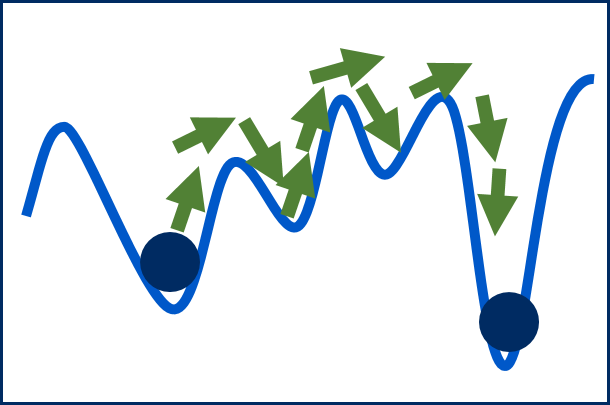
\includegraphics[bb=0 0 140 90, width=3.5cm]{normal_search.png}}
\hspace{5mm}
\subfigure[制約条件を考慮した探索]{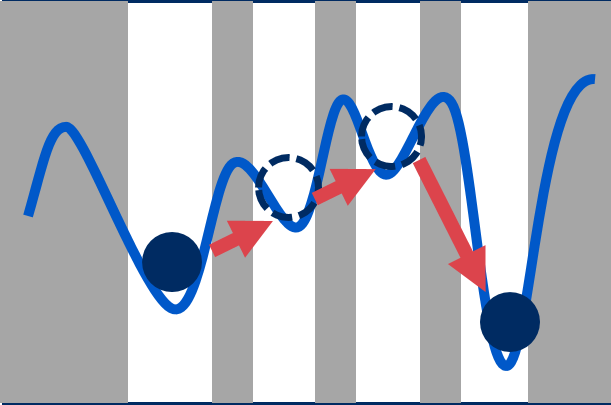
\includegraphics[bb=0 0 140 90, width=3.5cm]{va_search.png}}
\caption{制約機能を持つ擬似量子アニーリングマシンによる解探索}
\label{va_search}
\end{figure}


\begin{sourcecode}[tb] % Figure環境と同様にhtbが使えます.pは使えません.
% \vspace{3mm}
\caption{制約機能の使用例}\label{code:nec_va}
\begin{lstlisting}
# 制約条件の情報を配列形式で定義
one_hot_list = [
    ['x[0][0]', 'x[0][1]', 'x[0][2]', 'x[0][3]'],
    ['x[1][0]', 'x[1][1]', 'x[1][2]', 'x[1][3]'],
    ['x[2][0]', 'x[2][1]', 'x[2][2]', 'x[2][3]'],
]

# モデル作成時に制約条件を入力
va_model = VectorAnnealing.model(qubo, offset, onehot=one_hot_list)
\end{lstlisting}
\vspace{5mm}
\end{sourcecode}

%4
\section{性能評価}

%4.1
\subsection{評価環境}
疑似量子アニーリングマシンにおける制約機能の有効性を明らかにするために, 制約機能を持つ疑似量子アニーリングマシンを用いた評価を行った. はじめに, NEC VAを用いて制約機能を指定する場合と, 制約機能を使用しない場合の比較を行い, 1つの疑似アニーリングマシンでの制約機能の有無についてその有効性を議論する。次に、異なるアニーリングマシンでの制約機能の有無について評価するために, 制約機能を有する疑似量子アニーリングマシンとしてNEC VA, 及びFujitsu DA, 標準的な疑似量子アニーリングマシンとしてFixstars Amplify AEを取り上げ, 制約機能の有効性を議論する.

本評価に用いた各擬似量子アニーリングマシンの仕様の一覧を表\ref{table_spec}に示す. NEC VAはオンプレミス環境での利用が可能であり, Fujitsu DA, 及びFixstars Amplify AEは共にクラウド環境からのみ利用可能である.

% NEC VAの制約機能を利用する場合, 探索方式の異なる制約活用探索, または制約充足探索を選択することができる. 制約活用探索では, 外部入力された制約条件を探索時のヒント情報として活用し, 近傍を選択する際に制約破壊している変数を1つ以上訂正することで効率的な探索を行う. 制約活用探索では, 制約条件によるペナルティ関数を導入する必要がある一方, ペナルティ関数の重みには比較的小さな値を指定することができる. これにより, 制約機能を指定しない場合と比較して高い精度の解を得ることができる. また, 制約充足探索では, 外部入力された全ての制約条件を完全に満たす状態の中から解探索を行う. 制約充足探索を指定する場合では, ペナルティ関数をQUBOに含める必要はなく, これによりペナルティ関数の重みの影響を一切受けず, 局所的な解探索が可能になる.

擬似量子アニーリングマシンの制約機能の有効性を評価するためのベンチマーク問題として, 異なる制約を含む4つの最適化問題(QAP, TSP, QKP, MIS)を用いた. 性能評価の指標として, 複数実行により得られる解精度分布, 及びTime to Solution (TTS)を用いる. ここで解精度とは, 各ベンチマーク問題の既知最適解における目的関数値からの誤差率により表すものとする. 例えば解精度1\%の場合, 最適解における目的関数の1\%の誤差の解が得られたことを表す. また, TTSはアニーリングの性能評価に一般的に用いられる性能尺度であり, 以下の式で表される.
\begin{equation}
{\rm{TTS}}(\tau, p_{R}) = \tau\frac{{\rm{ln}}(1-p_{R})}{{\rm{ln}}(1-p_{s}(\tau))} \label{tts_def}
\end{equation}
ここで, $\tau$は1回あたりの計算時間, $p_{R}$は目標精度の解を得る確率の閾値である. $p_{s}(\tau)$は実際にその計算時間で目標精度の解を得た正答確率であり, 評価では$p_{R}=0.99$とした. 
% 表\ref{table_target}に, 各ベンチマーク問題毎に設定した目標精度を示す. 目標精度の決め方として, 本評価では各ベンチマーク問題において, 制約機能を指定する場合に正答率が100\%に届く精度のうち最良の値を選択した. 
NEC VAを用いた評価において,制約機能使用の有無における解精度の比較を行った.解精度は, アニーリングの反復回数を十分大きく指定することにより得られたものを用いた. 複数の疑似量子アニーリングマシンによる評価では, 各ベンチマーク問題毎に設定した目標解精度が得られる場合のTTS, 及び解精度の比較を行った. また, 計算の実行回数として, NEC VA, 及びFixstars Amplify AEでは10回, Fujitsu DAでは最大5回とした.

\newlength{\myheight}
\setlength{\myheight}{0.8cm}

\begin{table*}[tb]
\centering
  \caption{各疑似量子アニーリングマシンの仕様.}
    \begin{tabular}{|c||c|c|c|c}
      \hline
      \parbox[c][\myheight][c]{0cm}{}
      & {NEC VA} & {Fujitsu DA} & {Fixstars Amplify AE}\\ \hline \hline
      求解方式 & Simulated Annealing & MCMC Parallel Tempering & Simulated Annealing\\ \hline
      利用形態 & オンプレミス & クラウド & クラウド\\ \hline
      動作プラットフォーム & X86 CPU & GPU & Nvidia A100\\ \hline
      最大ビット/スピン数 & 100,000以上 & 100,000以上 & 262,144\\ \hline
      ビット階調 & 32bits/64bits & 64bits & 32bits/64bits\\ \hline
      制約処理技術 & 1hot & 2way-1hot  & -\\ 
      {} & 不等式制約 & 不等式制約 & {}\\ \hline
  \end{tabular}
\label{table_spec}
\end{table*}

% \begin{table}[tb]
% \centering
%   \caption{NEC VA実行時のペナルティ関数の重みの設定}
%     \begin{tabular}{|c||c|c|c}
%       \hline
%       \parbox[c][\myheight][c]{0cm}{}
%       & {制約活用探索} & {ペナルティ関数}\\ \hline \hline
%       TSP & $0.04\alpha\sim0.05\alpha\,(\alpha={\rm Max}(d_{i,j}))$ & $\alpha$\\ \hline
%       QAP & $\beta\sim20\beta\,(\beta={\rm Max}(f_{i,j}d_{k,l}))$ & $n\beta$\\ \hline
%       QKP & - & $10^{5}$\\ \hline
%       MIS & 1.1 & 2.0 \\ \hline
%   \end{tabular}
% \label{table_weight}
% \end{table}

% \begin{table}[tb]
% \centering
%   \caption{各ベンチマーク問題におけるTTSの目標精度.}
%     \begin{tabular}{|c||c|c|c|}
%       \hline
%       \multirow{2}{*}{TSP} & ch150 & kroA200 & pr226\\
%       \cline{2-2} \cline{3-3} \cline{4-4}
%                               & 1\% & 5\% & 10\%\\ \hline
%       \multirow{2}{*}{QAP} & tai80b & tai100b & tai150b\\
%       \cline{2-2} \cline{3-3} \cline{4-4}
%                             & \multicolumn{3}{|c|}{1\%}\\ \hline
%       \multirow{2}{*}{QKP} & jeu\_100\_50\_1 & jeu\_200\_50\_1 & jeu\_300\_50\_1\\
%       \cline{2-2} \cline{3-3} \cline{4-4}
%                             & \multicolumn{3}{|c|}{最適解}\\ \hline
%       \multirow{2}{*}{MIS} & frb\_53\_24\_1 & frb\_59\_26\_1 & frb\_100\_40\\
%       \cline{2-2} \cline{3-3} \cline{4-4}
%                             & \multicolumn{3}{|c|}{最適解}\\ \hline
%     \end{tabular}
% \label{table_target}
% \end{table}

%4.2
\subsection{NEC VAによる制約機能の評価}

%4.2.1
% \subsubsection{制約を含まないMaxcutによる評価}
% \textcolor{blue}{図\ref{TTS_Maxcut_VA}に, MaxcutによるTTSの評価結果を示す. データセットとして, Gset\cite{gset}のうち3つのインスタンスを用いた. X軸は各インスタンス名を示しており, インスタンス名の数値が大きいほど変数量が大きい. Y軸は各インスタンスにおけるTTSを示しており, 値が小さいほど性能が高いことを表す. 図\ref{TTS_Maxcut_VA}より, 問題規模の増大に伴いTTSが増加していく傾向が見られる. この要因を考察するために, 解精度分布による評価を行う. 図\ref{Cost_Maxcut_VA}に, 図\ref{TTS_Maxcut_VA}と同実行により得られた解精度分布を示す. 図\ref{Cost_Maxcut_VA}より, 問題規模が増大した場合でも解精度は大きく変化しないことが分かる. 従って, TTSの悪化要因が問題規模の増加に伴う実行時間の増加に起因することが分かる. 実行時間が増加する要因として, 問題規模の増大とともに解空間が増大し, 低エネルギー解へ到達するまでの探索回数が増加したためだと考えられる.}

% \begin{figure}[t]
% \centering
% 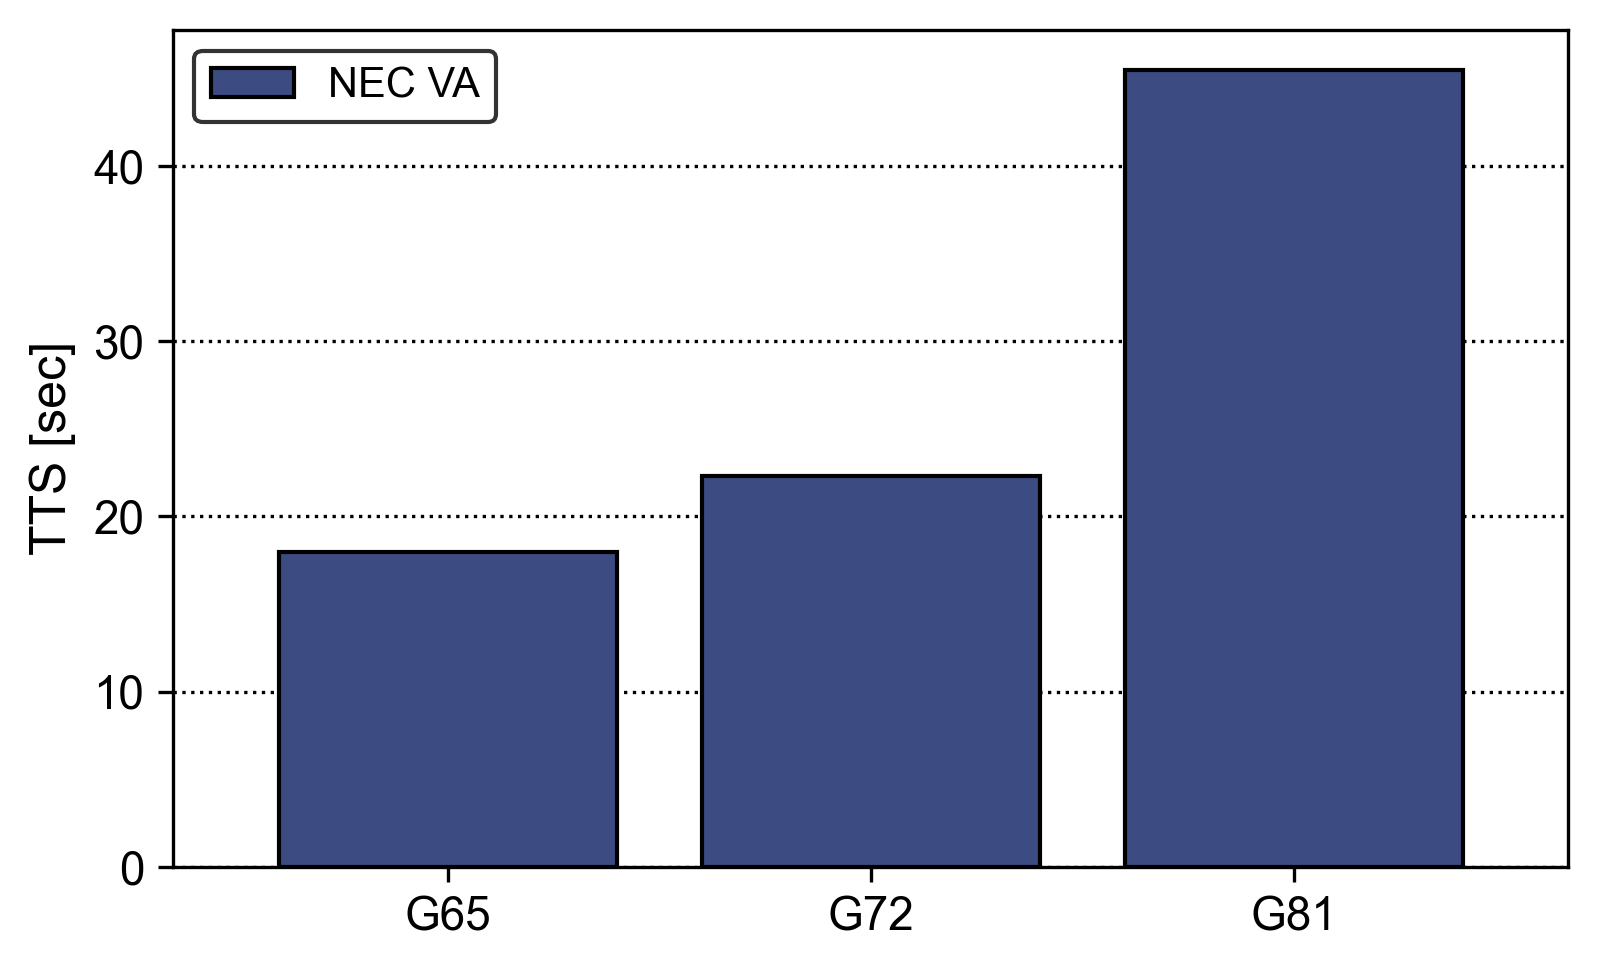
\includegraphics[bb=0 0 700 230, width=15cm]{TTS_Maxcut_VA.png}
% \caption{NEC VAによるTTSの比較(Maxcut).}
% \label{TTS_Maxcut_VA}
% \end{figure}

% \begin{figure}[t]
% \centering
% 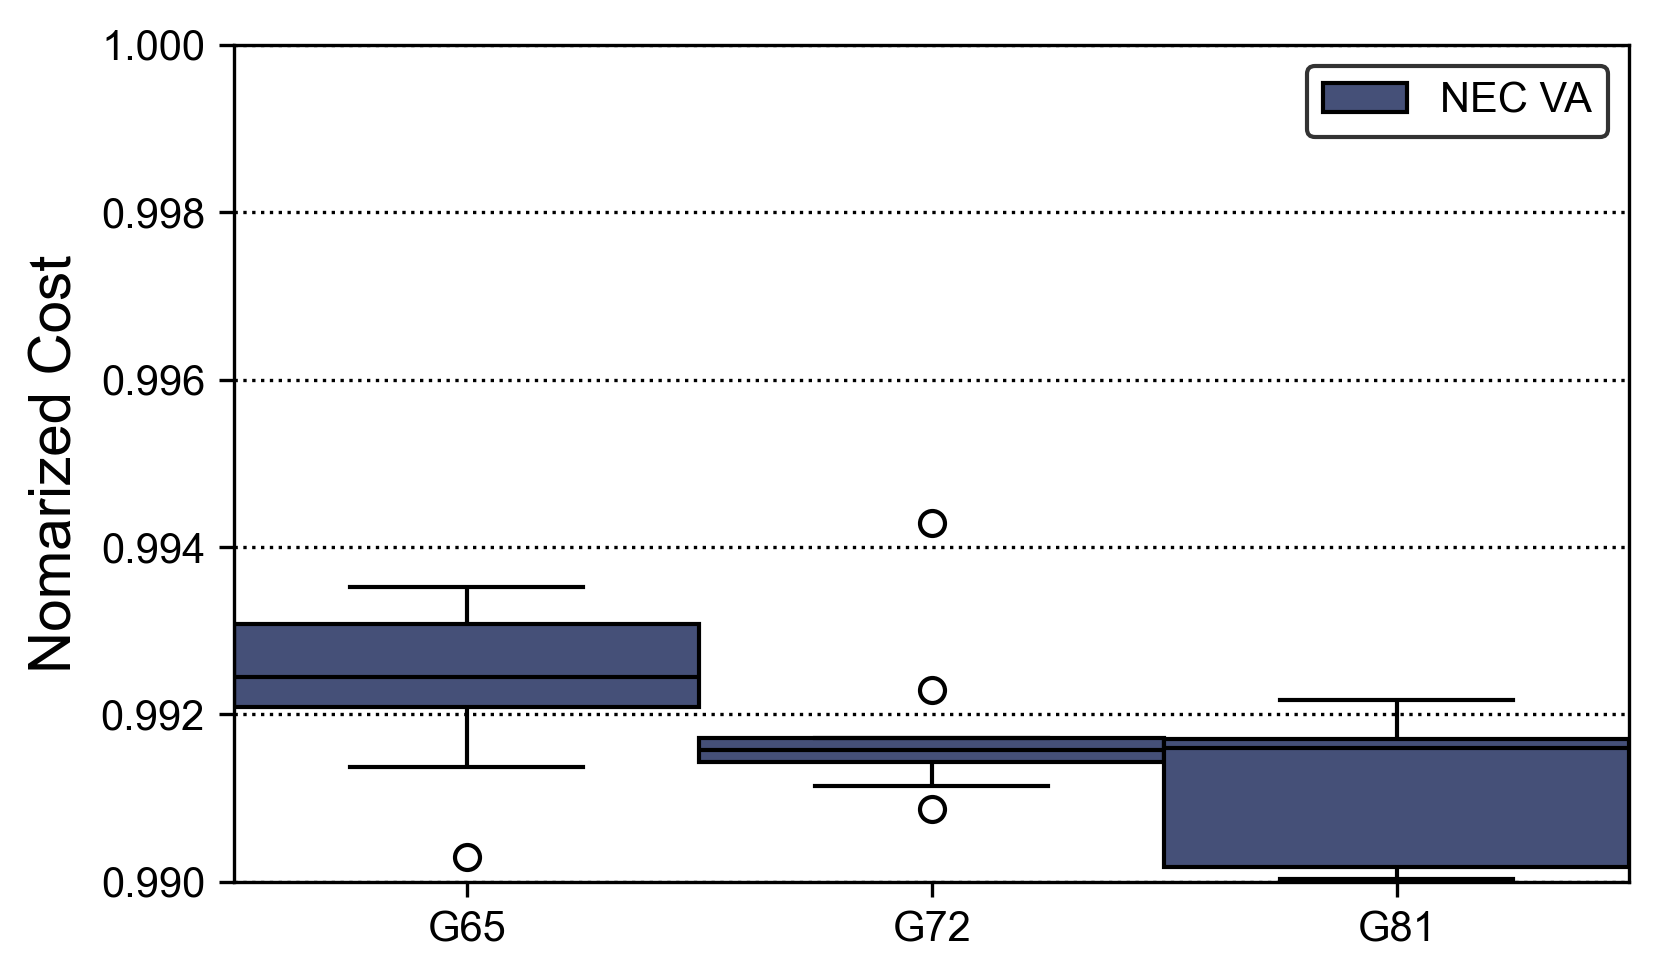
\includegraphics[bb=0 0 700 230, width=15cm]{Cost_Maxcut_VA.png}
% \caption{NEC VAによる解精度の比較(Maxcut).}
% \label{Cost_Maxcut_VA}
% \end{figure}

%4.2.2
\subsubsection{ワンホット制約を持つTSP, QAPによる評価}
図\ref{Cost_TSP_VA}に, TSPにおける解精度分布を示す. データセットとして, TSPLIB\cite{tsplib}のうち3つの都市データを用いた. 図\ref{Cost_TSP_VA}のX軸は各都市データ名を示しており, 都市データ名の数字は都市数を表し, その数値が大きいほど変数量が大きくなる. Y軸は各インスタンスにおける正規化された目的関数値を示しており, 値が小さいほど目的関数の精度が高く, 値が1となる場合に最適解に到達したことを表す. ここで, 制約機能を指定する場合では, 制約充足探索(constraint satisfaction), 及び制約活用探索(constraint utilization)による結果を示している. ここで, 制約充足探索では制約を満たした解のみを探索するのに対し, 制約活用探索では制約違反状態も経由し制約違反する変数が徐々に少なくなるように補助的な遷移を加えつつ探索する. また, 制約活用探索における制約重みの設定として, 目的関数の係数の最大値に0.05までの値を乗じた値を, 制約機能を使用しない場合(penalty function)では目的関数の係数の最大値をそれぞれ指定した.

図\ref{Cost_TSP_VA}より, 制約機能を使用しない場合, 制約機能を指定する場合と比較して全インスタンスで解精度が悪く, 解のばらつきも大きいことが分かる. これは, 制約機能を指定しない場合, 制約条件を満たすためにペナルティ関数の重みを大きく取らなければならず, 局所解近傍のエネルギー障壁が高くなり, 低エネルギー解への到達が難しくなったためである. これにより, 制約機能を指定しない場合では局所解へ陥りやすく, 解精度が悪化し, 解のばらつきも大きくなったと考えられる.
% また, 問題規模の増大に伴いエネルギー増減が激しくなることにより, 探索がさらに難しくなったと考えられる. 
一方, 制約機能を使用することにより, ワンホット制約を満たす有効解とその近傍を効率的に探索できるため, 制約機能を使用しない場合と比較して, 高い解精度を実現できていると考えられる.

また図\ref{Cost_TSP_VA}において, 制約処理方式の違いによる解精度は, 制約充足探索よりも制約活用探索の方が解精度が高い. これは, TSPでは目的関数の結合密度が小さく, 制約活用探索において導入するペナルティ関数の重みを十分小さく取れることに起因している. ペナルティ関数は目的関数の係数に対して重みが大きい場合, QUBOのエネルギー関数の形状が複雑化して局所解へ陥りやすくなる一方, 重みが小さい場合ではその形状が平易化され最適解への収束を容易にする効果が得られると考えられる. 制約活用探索と制約充足探索の結果の比較から, 制約活用探索では, エネルギーが低下した段階での遷移が活発になり, 高精度な解に収束しやすくなったと考えられる.

% \textcolor{blue}{二つの探索について, まず制約活用探索のみ目的関数にペナルティ関数を含めるという違いがある. ペナルティ関数は目的関数の重みに対し係数が大きい場合にQUBOのエネルギー地形を複雑化して局所解へトラップしやすくなる一方, 係数が小さい場合エネルギー地形を平易化して最適解への収束を補助する場合もあると考えらえる. 二つ目の違いとして制約充足探索では制約を満たした解のみ探索するのに対し, 制約活用探索では制約違反状態も経由し制約違反するスピンが徐々に少なくなるように補助的な遷移を加えつつ探索する違いがある. 以上を踏まえ結果を見ると制約活用探索はTSPにおいて小さい係数のペナルティ関数で制約を満たせているので, 制約充足探索と比較してエネルギーが下がった段階での遷移が活発になり良い解に収束したと考えられる.}

\begin{figure}[tb]
% \begin{figure}[tbp]
\centering
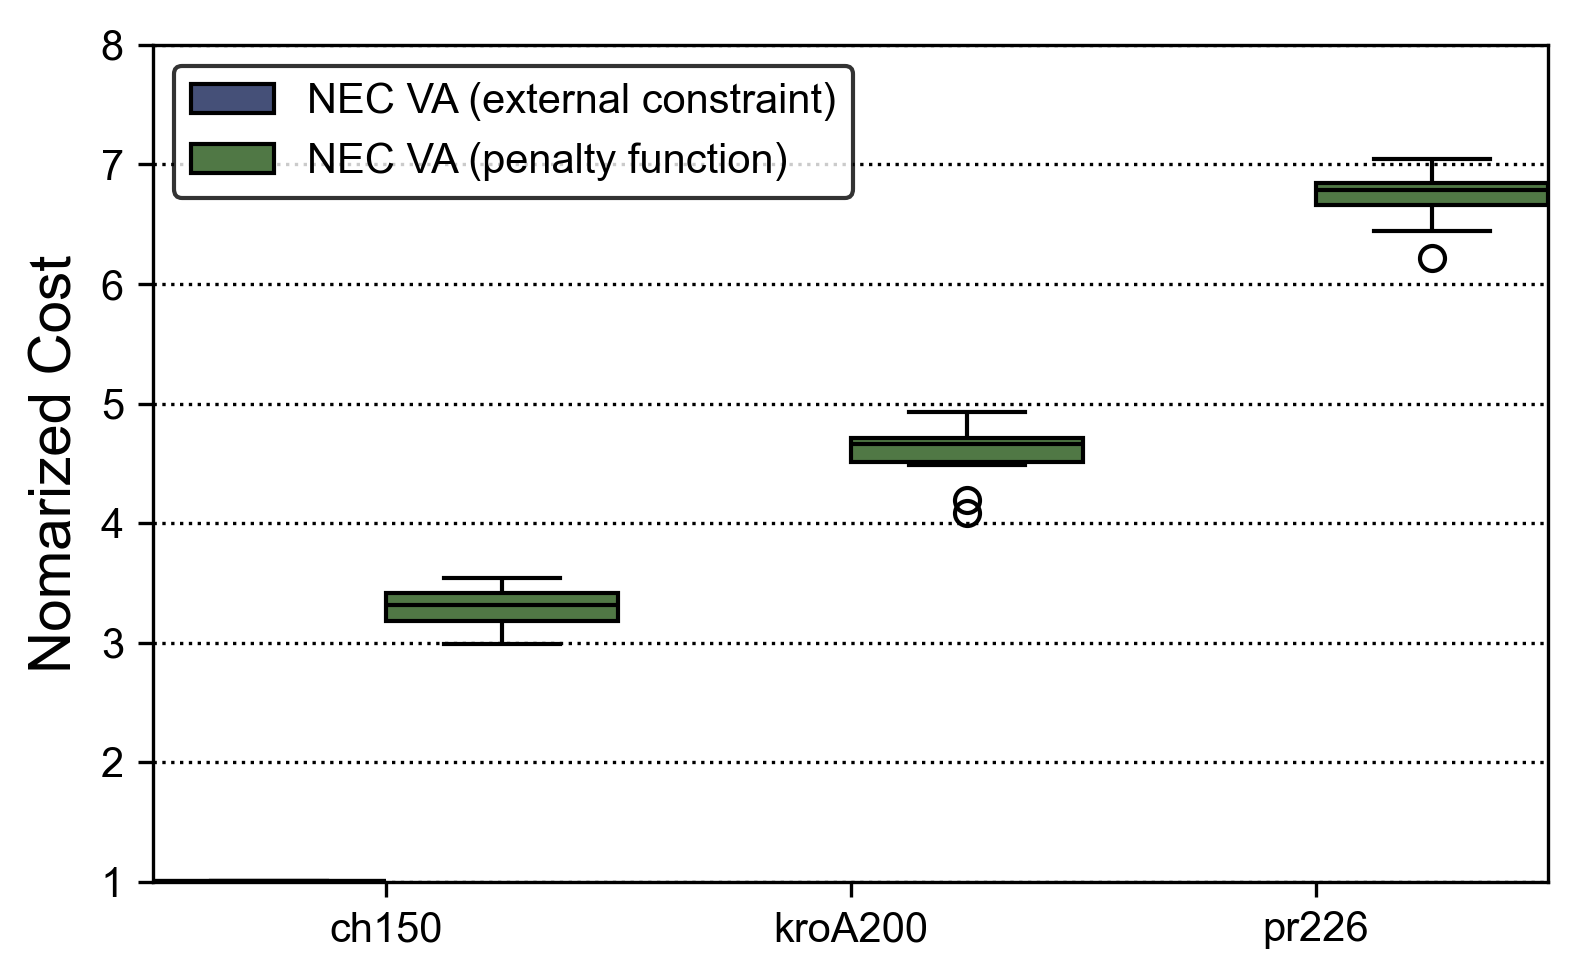
\includegraphics[bb=0 0 700 230, width=15cm]{Cost_TSP_VA.png}
\caption{NEC VAによる解精度の比較(TSP).}
\label{Cost_TSP_VA}
\end{figure}

図\ref{Cost_QAP_VA}に, QAPにおける解精度分布を示す. データセットとして, QAPLIB\cite{qaplib}のうち3つのデータを用いた. 図\ref{Cost_QAP_VA}のデータ名に含まれる数字はQAPの地点数を表しており, 数値が大きいほど変数量が大きくなる. また制約重みの設定として, 制約活用探索を指定する場合では目的関数の係数の最大値に20までの値を乗じた値を, 制約機能を使用しない場合では目的関数の係数の最大値に地点数を乗じた値をそれぞれ指定した.

図\ref{Cost_QAP_VA}より, 制約機能を使用しない場合, 制約機能を指定する場合と比較して全インスタンスで解精度が悪い. これは, TSPと同様に, ペナルティ関数を導入したことにより局所解近傍のエネルギー障壁が高くなり, 低エネルギー解への到達が難しくなったためである. 一方, 制約機能を使用することにより, 有効解とその近傍を効率的に探索できるため, 高い解精度に到達した.
% また, QAPにおいて制約条件を満たす有効解を得るためには, 問題規模の増大に応じてペナルティ関数に掛かる重みを大きく設定する必要がある\cite{qaplib}. これにより, 大規模問題ではペナルティ関数によるエネルギー関数の変動が大きくなり, 探索精度により影響を与えたと考えられる. 一方, 制約機能を指定することにより, 解空間を限定できる上, 大規模でもペナルティ関数の影響を受けることなく効率的に探索できるため, 高い解精度に到達できたと考えられる. }

また図\ref{Cost_QAP_VA}において, 制約処理方式の違いによる解精度は, 制約活用探索よりも制約充足探索の方が高い精度の解に到達している. この要因として, 制約活用探索において追加するペナルティ関数の重みが大きいことに起因していると考えられる. QAPでは, TSPと比較してペナルティ関数の重みを大きく取らなければ制約条件を満たす解が得られない. これは, TSPと比べてQAPではQUBOの結合密度が高く, 制約破壊時のエネルギー減少が大きくなりやすいことから, それに合わせた重みが必要になるためである. このため, 制約活用探索では大きな制約重みを指定した影響によりエネルギー関数の形状が複雑になり, 制約充足探索よりも早い段階で局所解に陥ったことで解精度の低下に繋がったと考えられる. 一方, 制約充足探索では, QUBOの中にペナルティ関数が含まれず, その重みによる影響を一切受けないことから, 高精度の解へ到達できたと考えられる.

% \textcolor{blue}{TSPの考察で見たように制約活用探索はペナルティ関数を追加する必要があるが, QAPの場合はこの係数を比較的大きくしなければ制約を満たせない. 理由として, TSPに対し重み係数の分散が大きく項も多いので, 制約破壊時のエネルギー変化が大きくなりやすくそれに合わせた係数のペナルティ関数が必要になることが考えられる. そのためペナルティ関数がエネルギー地形を複雑化し, 制約充足探索よりも早い段階で局所解にトラップしたことで悪い結果になったと考えられる. また制約充足探索においてもTSPに対しQAPでは解精度が良い. 制約は同じツーウェイワンホットであるため目的関数の差, 例えばQUBO行列の密度や重み係数の分散の違いが影響している可能性がある. }

\begin{figure}[tb]
% \begin{figure}[tbp]
\centering
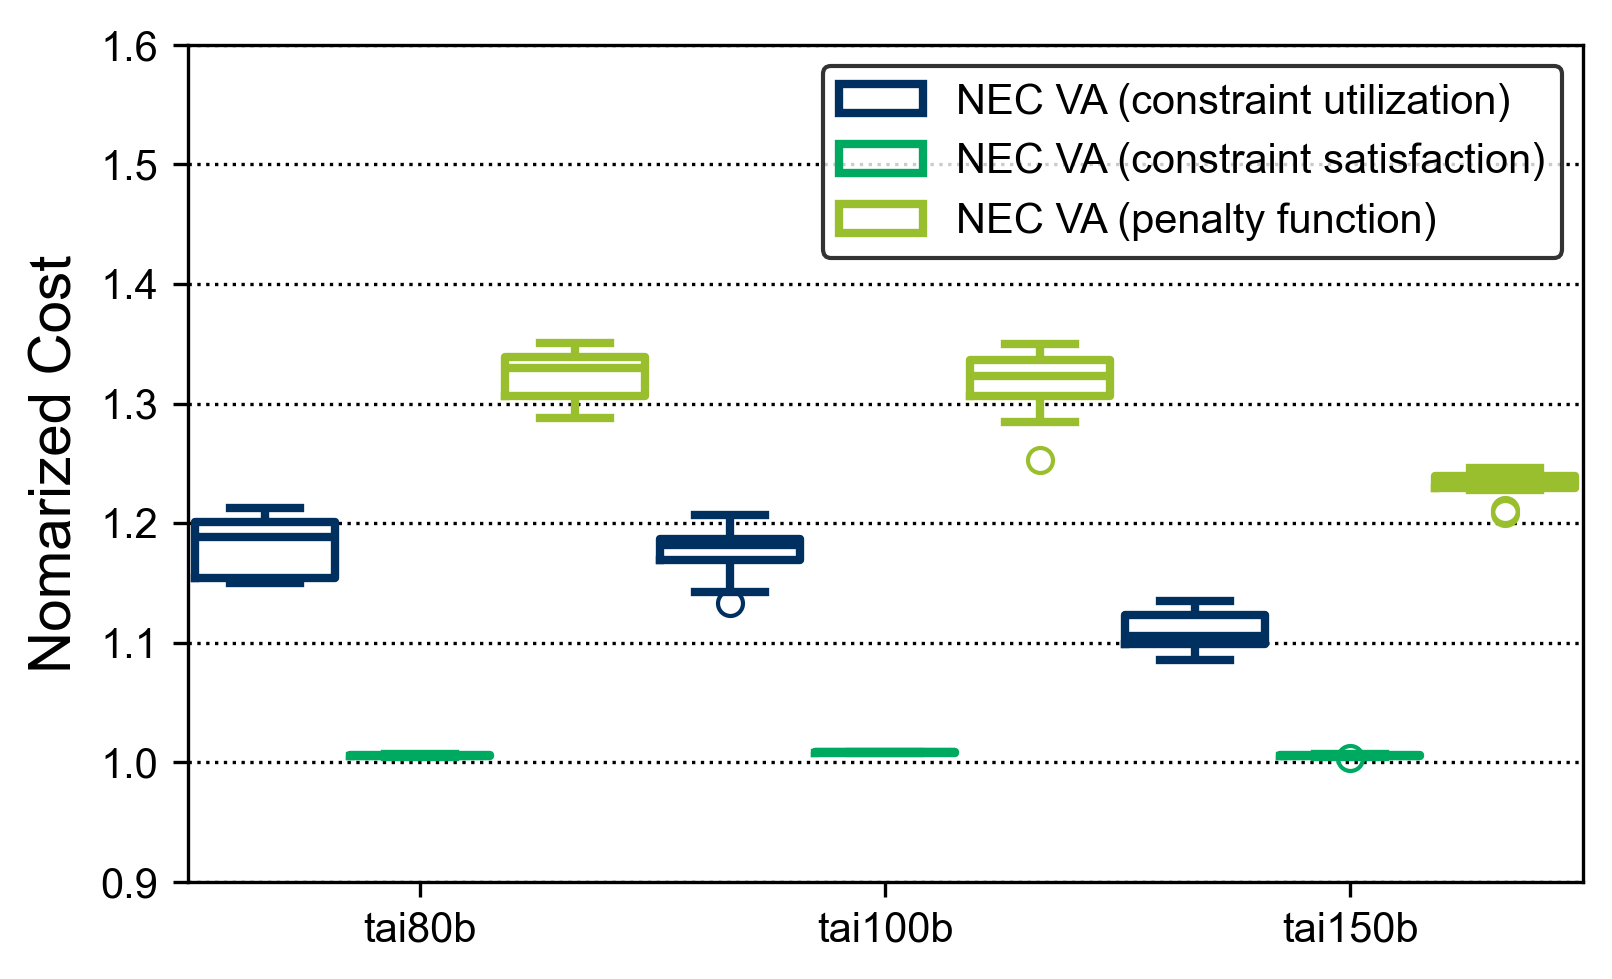
\includegraphics[bb=0 0 700 230, width=15cm]{Cost_QAP_VA.png}
\caption{NEC VAによる解精度の比較(QAP).}
\label{Cost_QAP_VA}
\end{figure}

%4.2.3
\subsubsection{不等式制約を持つQKPによる評価}
図\ref{Cost_QKP_VA}に, QKPにおける解精度分布を示す. データセットとして, 先行研究で作成されたデータ\cite{qkplib}のうち3つのデータを用いた. 図\ref{Cost_QKP_VA}のデータ名に含まれる3つの数字は左からそれぞれ, 変数量, QUBO の結合密度, 及びデータの種類を示している. また, 制約機能を指定する場合では, 不等式制約が提供されている制約充足探索による結果のみを示している. 制約機能を使用しない場合では, 制約重みに$100000$を指定した.

図\ref{Cost_QKP_VA}より, 制約機能を指定する場合では全インスタンスで最適解が得られている一方, 制約機能を使用しない場合では解精度が悪いことが分かる. この要因として, 不等式制約のペナルティ関数を導入する場合, エネルギー関数の変動に加えて, ペナルティ関数の導入過程で補助変数が追加されたことにより探索空間が増大し, 解精度に悪影響を与えたと考えられる. 一方, 制約充足探索を使用した場合, エネルギー関数にはペナルティ関数及び補助変数が含まれず, これらの影響を回避できたため, 高い精度の解が得られたと考えられる.

\begin{figure}[tb]
% \begin{figure}[tbp]
\centering
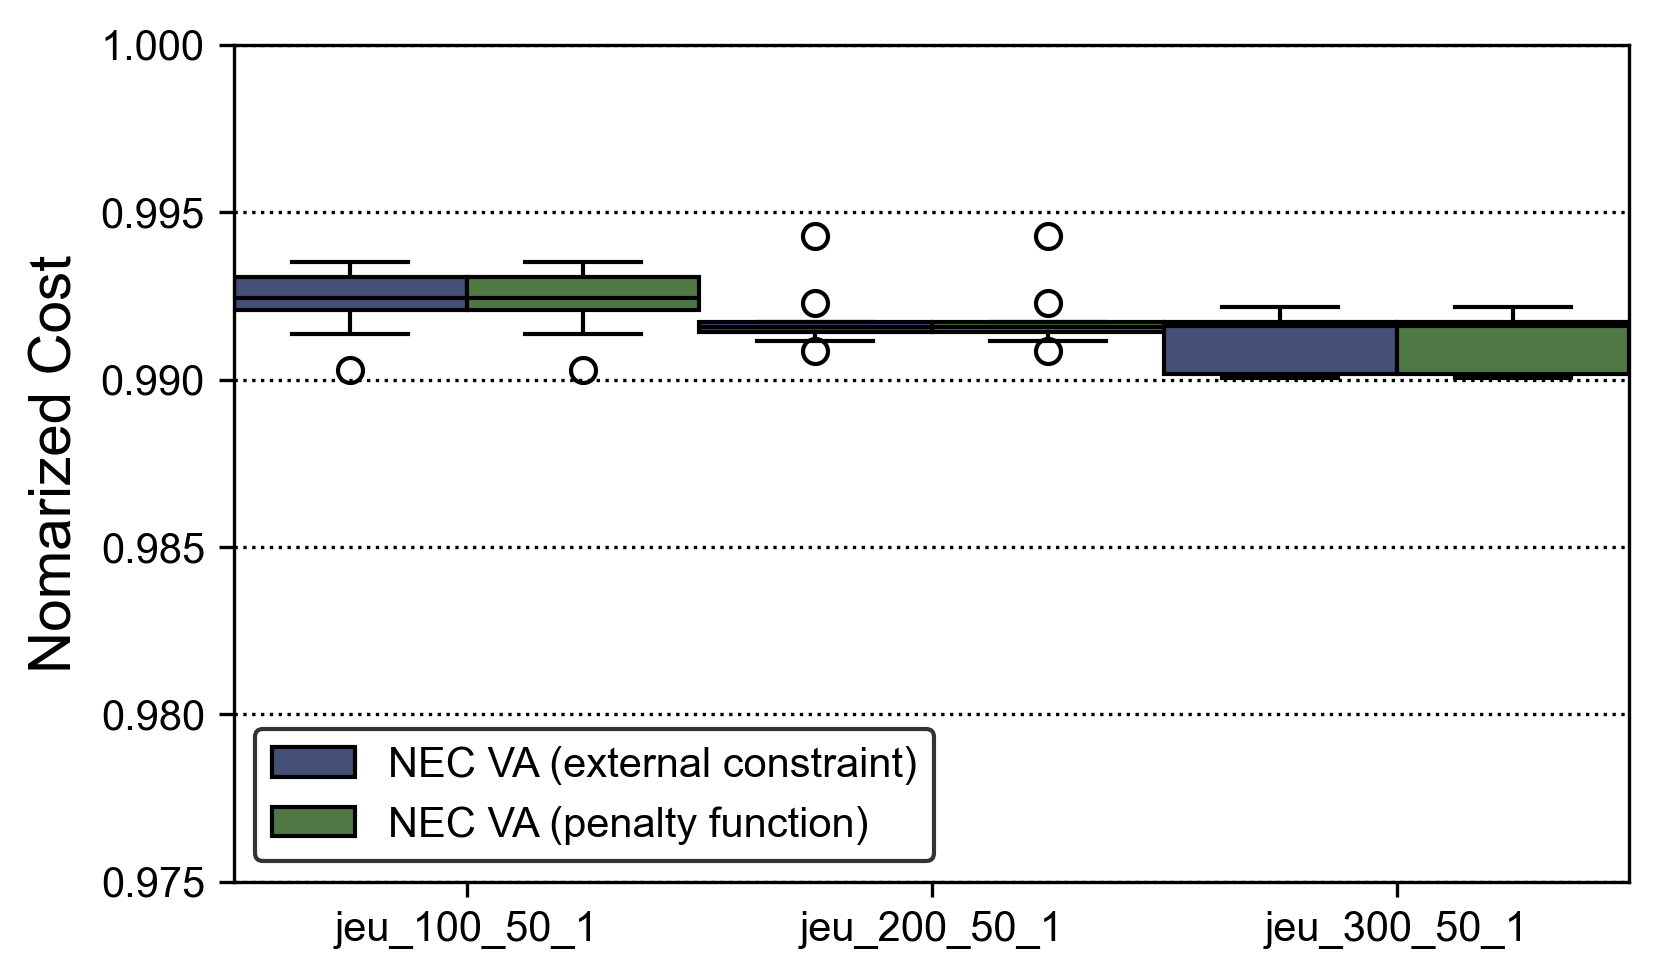
\includegraphics[bb=0 0 700 230, width=15cm]{Cost_QKP_VA.png}
\caption{NEC VAによる解精度の比較(QKP).}
\label{Cost_QKP_VA}
\end{figure}
% 【図は上、表は上か下】

%4.2.4
\subsubsection{禁止ペア制約を持つMISによる評価}
図\ref{Cost_MIS_VA}に, MISにおける解精度分布を示す. データセットとして, BHOSLIB\cite{mislib}のうち3つのデータを用いた. 図\ref{Cost_MIS_VA}の各データ名のfrbに含まれる数字の値が大きいほど問題の変数量が大きいことを示している. また制約重みの設定として, 制約活用探索を指定する場合では1.1, 制約機能を使用しない場合では2.0を指定した.

図\ref{Cost_MIS_VA}より, MISでは, 制約機能を使用する場合, 及び制約機能を使用しない場合ともに, 全インスタンスで最適解に到達している. 禁止ペア制約において制約機能を使用しない場合に高い精度を実現できる要因として, MISの目的関数は対称かつ単調な一次式で構成されることから, 禁止ペア制約をペナルティ関数として追加した場合においても局所解に陥ることが殆どなく, 高い解精度を維持できたためだと考えられる. 従ってMISにおいては, 制約機能を使用せずに, 制約をペナルティ関数として導入する場合においても高い解精度が得られることが分かった.

% \textcolor{blue}{また, 制約機能を使用する場合, 及び制約機能を使用しない場合における最適解に到達するまでの実行時間を比較するために, 図\ref{TTS_MIS_VA}に同実行により得られたTTSを示す. 図\ref{TTS_MIS_VA}のY軸は各インスタンスにおけるTTSを示しており, 値が小さいほど短時間で高確率に最適解が得られたことを表す. ここで, MISでは制約機能を使用する場合, 及び制約機能を使用しない場合ともに正答率100\%で最適解が得られていることから, 図\ref{TTS_MIS_VA}のTTSは各インスタンスにおける実行時間と等しい. 図\ref{TTS_MIS_VA}に示す通り, TTSは制約機能を使用する場合の方が大きい. これは, MISでは禁止ペア制約の項数が多く, 探索毎に外部指定された各制約を満たしているかを判断する必要があることから一探索当たりの実行時間が長くなったためである.} 一方で, 制約機能を使用しない場合では, 禁止ペア制約の項数が増加した場合でもペナルティ関数の係数がQUBOに埋め込まれるのみであるため, 実行時間に大きく影響しないと考えられる.

以上の制約機能有無による評価結果から,制約条件を含むベンチマーク問題においては殆どの場合において制約機能が有効であることを明らかにした.一方,MISのように, ペナルティ関数をQUBOに埋め込んで求解することの処理コストが十分に小さい制約を含む問題においては,制約機能を使用せずに, ペナルティ関数を導入しても, 高い解精度が得られる場合もあることが確認できた.

\begin{figure}[tb]
% \begin{figure}[tbp]
\centering
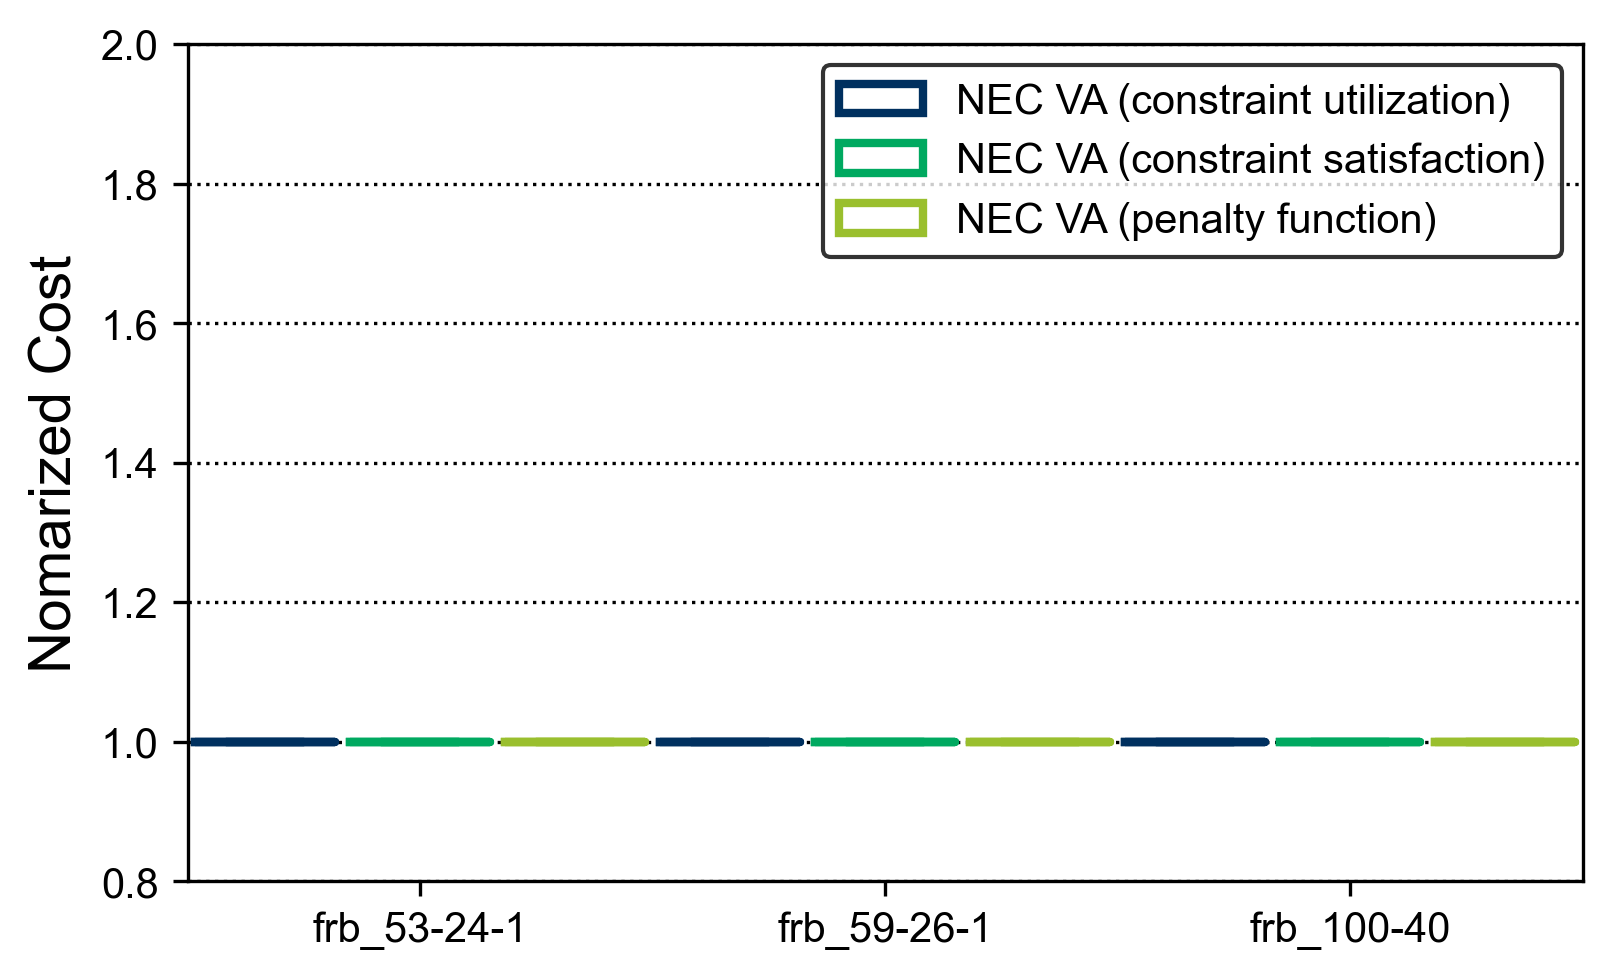
\includegraphics[bb=0 0 700 230, width=15cm]{Cost_MIS_VA.png}
\caption{NEC VAによる解精度の比較(MIS).}
\label{Cost_MIS_VA}
\end{figure}

% \begin{figure}[tb]
% % \begin{figure}[tbp]
% \centering
% 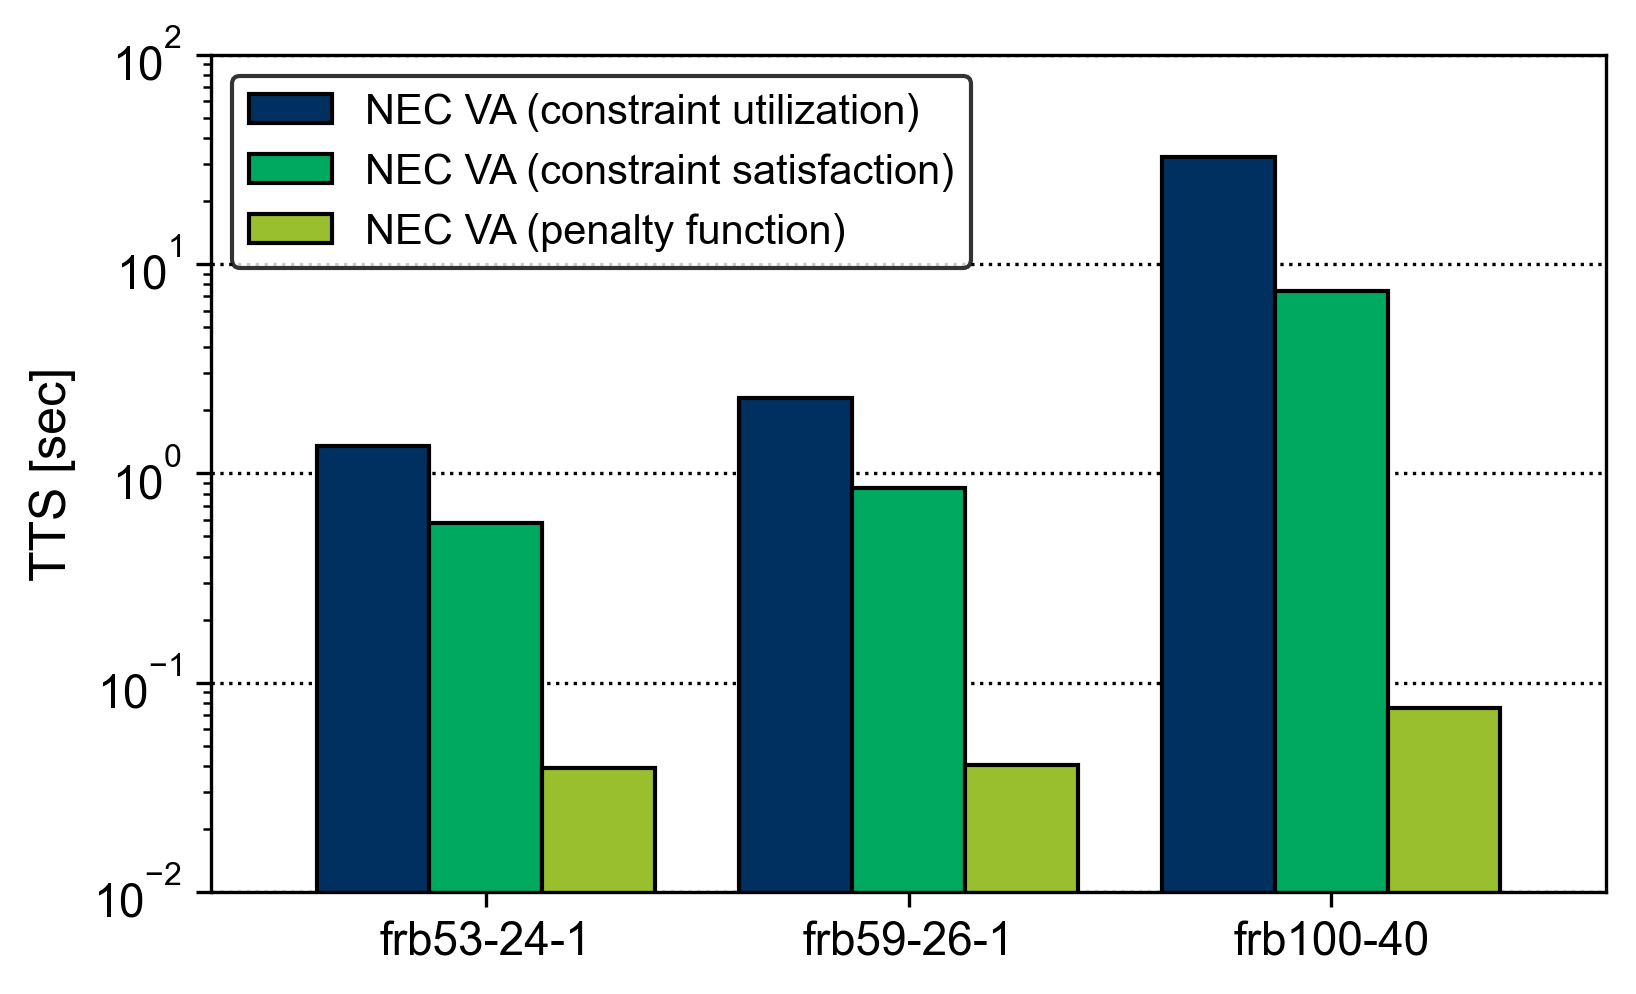
\includegraphics[bb=0 0 700 230, width=15cm]{TTS_MIS_VA.png}
% \caption{NEC VAによるTTSの比較(MIS).}
% \label{TTS_MIS_VA}
% \end{figure}

\subsection{異なる疑似量子アニーリングマシンを用いた評価}
本節では, 擬似量子アニーリングマシンの制約機能の有効性を検証するために, NEC VA, Fujitsu DA, 及びFixstars Amplify AEを用いた評価結果について述べる. 本評価において, NEC VA, 及びFujitsu DAでは制約機能を指定し, Fixstars Amplify AEでは制約条件をペナルティ関数として導入した. 以下に制約条件を含まないMaxcut, 及び4.2節で用いた4つの最適化問題による結果を述べる. 性能の指標として解精度, 及びTTSを使用し, TTSの目標精度としてMaxcut, 及びQAPでは1\%, TSPでは20\%, QKP, 及びMISでは最適解とした. また, NEC VAの制約処理方式として, 各ベンチマーク問題に応じて高い精度が得られた探索方式を採用した.

% \begin{table}[tb]
% % \begin{table}[tbp]
% \centering
%   \caption{各ベンチマーク問題におけるTTSの目標精度.}
%     \begin{tabular}{|c|c|c|c|c|}
%       \hline
%       G81 & pr226 & tai150b & jeu\_300\_50\_1 & frb\_100\_40\\
%       (Maxcut) & (TSP) & (QAP) & (QKP) & (MIS)\\
%       \cline{1-1} \cline{2-2} \cline{3-3} \cline{4-4} \cline{5-5}
%        1\% & 20\% & 1\% & \multicolumn{2}{|c|}{最適解}\\ \hline
%     \end{tabular}
% \label{table_target2}
% \end{table}

図\ref{TTS_All}に, 各擬似量子アニーリングマシンによる, 各ベンチマーク問題で用いた最大規模のデータによるTTSを示す. 図\ref{TTS_All}においてTTSの結果が表示されていない場合, そのインスタンスにおいて目標精度の解が得られなかったことを意味している. 図\ref{TTS_All}に示す通り, Maxcut G81を除く制約条件を含む問題では, Fixstars Amplify AEに対してNEC VA, 及びFujitsu DAのTTSが小さく, Fixstars Amplify AEではQAP tai150b, 及びQKP jeu\_300\_50\_1において目標精度の解が得られていない. 

また, TSP pr226, 及びQAP tai150bにおけるNEC VAとFujitsu DAの結果を比較した場合, TSP pr226ではNEC VA, QAP tai150bではFujitsu DAの方がTTSが小さいことが分かる. 同一の制約条件を持つ問題においてNEC VAとFujitsu DAのTTSが逆転する要因として, TSPとQAPにおけるペナルティ関数の重みの大きさの違い, 及びNEC VAとFujitsu DAの制約機能における探索処理の実装の違いが影響していると考えられる. Fujitsu DAの制約機能を指定する場合, NEC VAの制約充足探索と同様に, ペナルティ関数をQUBOに含める必要がない. また, Fujitsu DAのtwo\_way\_one\_hot\_groupsを指定した場合, ツーウェイワンホット制約を満たす局所的な状態の中から解探索が行われる. このため, ペナルティ関数の重みを小さく指定できるTSP pr226では制約活用探索によって比較的良い解への収束が容易になるNEC VAのTTSが小さくなる. 一方で, ペナルティ関数の重みを大きくせざるを得ないQAP tai150bではペナルティ関数が不要なNEC VAの制約充足探索とFujitsu DAのtwo\_way\_one\_hot\_groupsによる比較となるが, 探索処理の実装上の違いから実行時間に差がありFujitsu DAのTTSが小さくなっている.

また図\ref{Cost_All}に, 同実行により得られた解精度分布を示す. 図\ref{Cost_All}より, Maxcut G81, 及びMIS frb\_100\_40では, 各疑似量子アニーリングマシンの制約機能の有無によらず, 全実行で目標精度の解に到達していることが分かる. 一方で, TSP pr226, QAP tai150b, 及びQKP jeu\_300\_50\_1では, Fixstars Amplify AEにおける全実行のうち目標精度の解に到達しない解の割合が大きくなる. このため, NEC VAによる制約機能の有効性評価で見られた傾向と同様に, ワンホット制約, 及び不等式制約を持つ問題においては, 疑似量子アニーリングマシンの制約機能を指定する場合が, 制約機能を指定しない場合に対して高い求解精度を実現できることが確認された. 一方で, 禁止ペア制約を含むMIS frb\_100\_40においては, 制約条件をペナルティ関数として導入した場合においても処理コストが十分に小さく, 制約機能を持たないFixstars Amplify AEにおいても十分に高い解精度が得られることが検証できた. 

% \begin{figure}[tbp]
\begin{figure}[tb]
\centering
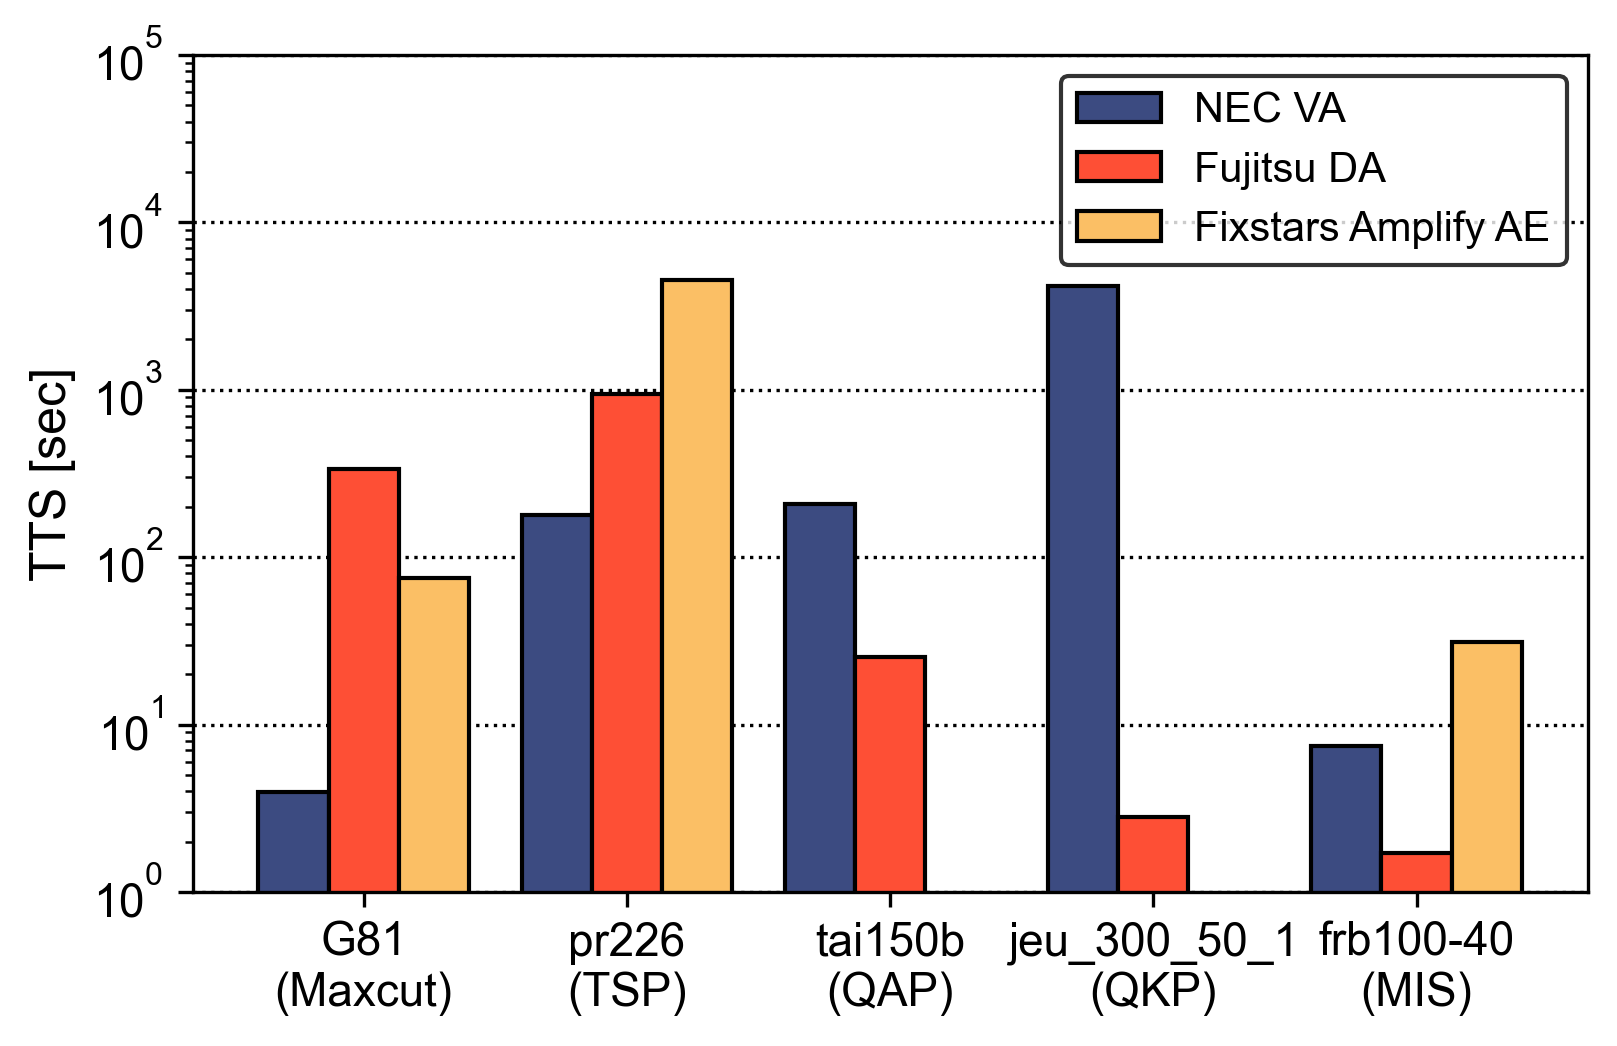
\includegraphics[bb=0 0 700 230, width=15cm]{TTS_All.png}
\caption{擬似量子アニーリングマシンによるTTSの比較.}
\label{TTS_All}
\end{figure}

% \begin{figure}[tbp]
\begin{figure}[tb]
\centering
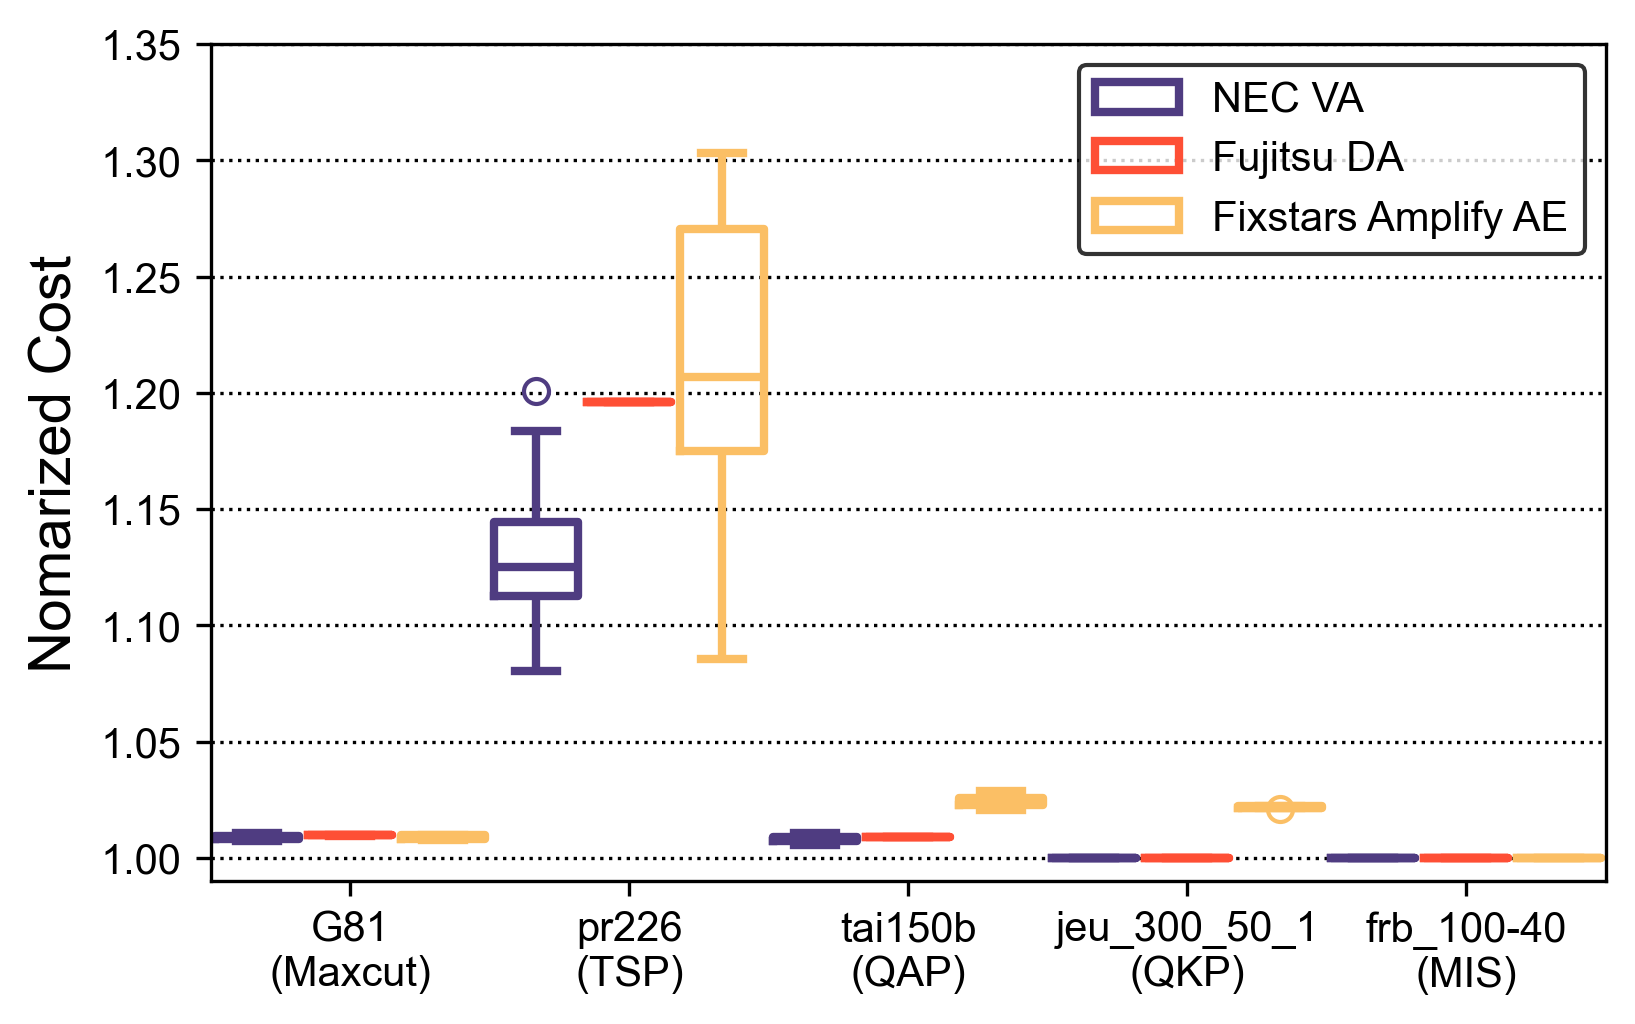
\includegraphics[bb=0 0 700 230, width=15cm]{Cost_All.png}
\caption{擬似量子アニーリングマシンによる解精度の比較.}
\label{Cost_All}
\end{figure}

%6
\section{おわりに}
本稿では, 制約条件を含まないMaxcut, 及び異なる制約条件を含むTSP, QAP, QKP, MISを用いて, 擬似量子アニーリングマシンの制約機能の評価を行った. 結果として, ワンホット制約を含むQAP, TSP, 及び不等式制約を含むQKPでは, 擬似量子アニーリングマシンの制約機能を指定した場合に, 制約機能を使用しない場合と比較して高い解精度を実現できることが分かった. 一方, 禁止ペア制約を含むMISでは, 問題が単純な式で表現可能であり, QUBOにペナルティ関数を導入しても局所解に陥ることが殆どなく, 制約機能を持たない擬似量子アニーリングマシンにおいても十分に高い解精度が得られることを示した. また, 制約機能を持つ異なる擬似量子アニーリングによる評価結果から, 各擬似量子アニーリングマシンにおける制約機能の実装の違いと各ベンチマーク問題における目的関数と制約条件の性質がTTSに影響を与えることが分かった. これらの結果から, 疑似量子アニーリングマシンの制約機能が求解性能に大きく寄与しており, 各問題に応じて適切な制約機能を使用することが重要であることを明らかにした.

\begin{acknowledgment}
本研究の一部は,文部科学省「次世代計算基盤に係る調査研究」新計算原理調査研究,科研費 \#22KK0181, \#23K28088の助成を受けて実施している. また, 国立研究開発法人新エネルギー・産業技術総合開発機構 (NEDO) の委託業務 (JPNP23003)を受けて実施している.
\end{acknowledgment}

\begin{thebibliography}{10}

\bibitem{jobshop}
C. Carugno, Maurizio, F. Dacrema, and Paolo Cremonesi, Evaluating the job shop scheduling problem on a D-wave quantum annealer, {\it Scientific Reports}, {\bf 12}, 6539 (2022).

\bibitem{isc-onoda}
M. Onoda, K. Komatsu, K. Bannai, S. Momose, M. Sato, and H. Kobayashi, Performance Evaluation of Vector Annealing  on Multiple Nodes using  the Traveling Salesperson Problem, {\it International Supercomputing Conference (ISC)} (2025).

\bibitem{portfolio}
W. Sakuler, J. M. Oberreuter, R. Aiolfi, L. Asproni, B. Roman, and J. Schiefer, A real-world test of portfolio optimization with quantum annealing, {\it Quantum Machine Intelligence }, {\bf 7}, 43 (2025).

\bibitem{tsunami}
Y. Liu, K. Komatsu, M. Kumagai, M. Sato, and H. Kobayashi, Performance Evaluation of Tsunami Evacuation Route Planning on Multiple Annealing Machines, {\it CF '23: Proceedings of the 20th ACM International Conference on Computing Frontiers}, 185 - 188 (2023).

\bibitem{ml}
K. Aoyama, K. Komatsu, M. Kumagai, and H. Kobayashi, Analysis of Precision Vectors for Ising-Based Linear Regression, {\it Parallel and Distributed Computing, Applications and Technologies}, 251–261 (2023).

\bibitem{nishimori}
T. Kadowaki and H. Nishimori, Quantum annealing in the transverse Ising model, {\it Phys. Rev. E}, {\bf 58}, 5355-5363 (1998).

\bibitem{d-wave}
M. W. Johnson, {\it et al}, Quantum annealing with manufactured spins, {\it Nature}, {\bf 473}, 194–198 (2011).

\bibitem{takano}
鷹野芙美代, 鈴木基己, 小林悠記, 荒木拓也. 組合せ最適化問題における制約条件を考慮したQUBOソルバ, {\bf 119}, 314, 15-20 (2019).

\bibitem{Lucas} 
A. Lucas, Ising formulations of many np problems, {\it Frontiers in physics}, {\bf 2}, 5 (2014).

\bibitem{yatabe}
A. Yatabe, Partitioning QUBO with two-way one-hot conditions on traveling salesman problems for city distributions with multiple clusters, {\it Frontiers in Computer Science}, {\bf 6}, 1285244 (2024).

\bibitem{maxcut}
F. Glover and G. Kochenberger, A Tutorial on Formulating QUBO Models Version 1 (2018).

\bibitem{gset}
Gset, https://web.stanford.edu/~yyye/yyye/Gset/.

\bibitem{tsplib}
G. Reinelt, Tsplib|a traveling salesman problem library, {\it FORSA journal on computing}, {\bf 3}, 376 (1991).

\bibitem{qaplib}
R.E. Burkard, S. Karisch and F. Rendl, QAPLIB – A Quadratic Assignment Problem Library, {\it Journal of Global Optimization}, {\bf 10}, 391-403 (1997).

\bibitem{qkplib}
É. Soutif and A. Billionnet, An exact method based on Lagrangian decomposition for the 0–1 quadratic knapsack problems, {\it Eur.J.Oper.Res.}, {\bf 157}, 3, 565–575 (2024).

\bibitem{mislib}
BHOSLIB, https://networkrepository.com/bhoslib.php

\bibitem{va} 
NEC Corporation, 今ある最適化問題解決に - NEC Vector Annealing, https://jpn.nec.com/nec-vector-annealing-service/index.html.

\bibitem{da}
M. Aramon, G. Rosenberg, E. Valiante, T. Miyazawa, H.Tamura,and H.G.Katzgraber, Physics-inspired optimization for quadratic unconstrained problems using a digital annealer, {\it Frontiers in Physics}, {\bf 7}, 48 (2019).

\bibitem{amplify}
Fixstars Corporation, Annealing Machines - The Quantum Computing Cloud - Fixstars Amplify, https://amplify.fixstars.com/en/engine.

\bibitem{kumagai}
M. Kumagai, K. Komatsu, F. Takano, T. Araki, M. Sato, H. Kobayashi, An External Definition of the One-Hot Constraint and Fast QUBO Generation for High-Performance Combinatorial Clustering, {\it International Journal of Networking and Computing}, {\bf 11}, 2 (2021).

\bibitem{komatsu}
K. Komatsu, M. Kumagai, J. Qi, M. Sato, and H. Kobayashi, An externally-constrained ising clustering method for material informatics, {\it 2021 Ninth International Symposium on Computing and Networking Workshops (CANDARW)}, 201–204 (2021).

\bibitem{komatsu2}
K. Komatsu, Makoto. Onoda, M. Kumagai, and H. Kobayashi, Investigating the Characteristics of Ising Machines, {\it 2023 IEEE International Conference on Quantum Computing and Engineering (QCE)} (2023).

\bibitem{kumagai2}
M. Kumagai, K. Komatsu, F. Takano, T. Araki, M. Sato, and H. Kobayashi, Combinatorial clustering based on an externally-defined one-hot constraint, {\it Eighth International Symposium on Computing and Networking (CANDAR)}, 59–68 (2020).

\bibitem{da2}
M. Aramon, G. Rosenberg, E. Valiante, T. Miyazawa, H. Tamura and H. G. Kartzgraber, Physics inspired optimization for quadratic unconstrained problems using a Digital Annealer, {\it Frontiers in Physics}, {\bf 7}, 48 (2019).

\bibitem{da3}
K. Kanda, H. Tamura, M. Begherbeik, P. Ashtari, S. Mousavi and A. Sheikholeslami, イジング最適化を用いた二次割当問題の高速求解, {\it Abstracts. Spring National Conference of Operations Research Society of Japan}, {\bf 2022}, 24-25 (2022).

\bibitem{amplify-da}
P. Codognet, D. Diaz, and S. Abreu, Quantum and Digital Annealing for the Quadratic Assignment Problem, {\it 2022 IEEE International Conference on Quantum Software (QSW)}, 1-8 (2022).

\bibitem{ozeki}
S. Hirama and M. Ohzeki, Efficient Algorithm for Binary Quadratic Problem by Column Generation and Quantum Annealing, {\it Journal of the Physical Society of Japan}, {\bf 92}, 11 (2023).

\bibitem{onoda2}
M. Onoda, K. Komatsu, M. Kumagai, M. Sato, H. Kobayashi, A Constraint Partition Method for Combinatorial Optimization Problems, {\it 2023 IEEE 16th International Symposium on Embedded Multicore/Many-core Systems-on-Chip (MCSoC)} (2023).

\end{thebibliography}

\end{document}
